\documentclass[twoside,spanish,11pt]{book}

\usepackage[utf8]{inputenc}
\usepackage[T1]{fontenc}
\usepackage[spanish,es-tabla,english]{babel}

\usepackage[usenames, dvipsnames]{xcolor}

\usepackage{array}
\usepackage{subcaption}
\usepackage[toc,page]{appendix}
\usepackage{multirow}
\usepackage{indentfirst}
\usepackage{cite}

\usepackage{ulem}
\renewcommand{\uline}[1]{\textit{#1}}
\definecolor{MyOrange}{rgb}{0.9,0.6,0.0}
\definecolor{MyDarkBlue}{rgb}{0,0,0.8}
\definecolor{MyDarkRed}{rgb}{0.6,0,0.0}
\newcommand{\borrar}[1]{\textcolor{MyDarkRed}{\sout{#1}}} %\sout}
\newcommand{\nuevo}[1]{\textcolor{MyDarkBlue}{\uline{#1}}} %\sout}
\newcommand{\nota}[1]{\textcolor{MyOrange}{#1}} %\sout}

\reversemarginpar
\usepackage{setspace}
\usepackage{todonotes}
\newcounter{mycomment}
\newcommand{\mycomment}[3][]{%
% initials of the author (optional) + note in the margin
    \refstepcounter{mycomment}%
    {%
        \setstretch{0.7}% spacing
        \todo[color=#3,size=\scriptsize]{%
            \tiny{\textbf{(\themycomment)[\uppercase{#1}]:}~#2}}%
    }}
% For notes, corrections and suggestions
\definecolor{GRCOLOR}{rgb}{1,0.2,0.5}
\definecolor{ODRCOLOR}{rgb}{0.2,0.75,0.25}
\definecolor{LRCOLOR}{rgb}{0.2,0.3,1}
\definecolor{MyDarkRed}{rgb}{0.6,0,0.0}

\newcommand{\GR}[1] { \mycomment[GR]{#1}{GRCOLOR}}
\newcommand{\ODR}[1]{ \mycomment[ODR]{#1}{ODRCOLOR}}
\newcommand{\LR}[1]{ \mycomment[LR]{#1}{LRCOLOR}}

\newcommand{\newGR}[1]{\textcolor{GRCOLOR}{\uline{#1}}} %\sout}
\newcommand{\delGR}[1]{\textcolor{GRCOLOR}{\sout{#1}}} %\sout}
\newcommand{\newODR}[1]{\textcolor{ODRCOLOR}{\uline{#1}}} %\sout}
\newcommand{\delODR}[1]{\textcolor{ODRCOLOR}{\sout{#1}}} %\sout}
\newcommand{\newLR}[1]{\textcolor{LRCOLOR}{\uline{#1}}} %\sout}
\newcommand{\delLR}[1]{\textcolor{LRCOLOR}{\sout{#1}}} %\sout}
\newcommand{\note}[1]{\textcolor{MyDarkRed}{#1}} %\sout}
\newcommand{\deletenote}[1]{\textcolor{MyDarkRed}{\sout{#1}}} %\sout}


%\newcommand{\delsg}[1]{\textcolor{SGCOLOR}{\sout{#1}}} %\sout}

\usepackage{graphicx}
\usepackage{listings}
\usepackage{float}

\usepackage{rotating}

\usepackage[hyphens]{url} % Hay que cargarlo antes que hyperref para URLs largas
\usepackage[hidelinks=true]{hyperref}
\hypersetup{
%	colorlinks,
    linkcolor={blue!80!black},
    citecolor={blue!80!black},
    urlcolor={blue!80!black}
}
%\hypersetup{
%    colorlinks,
%    linkcolor={black},
%    citecolor={black},
%    urlcolor={black}
%}

\usepackage{marginnote}
\renewcommand*{\marginfont}{\scriptsize\color{red}\sffamily}

\usepackage{enumitem}
\setitemize{noitemsep,topsep=0pt,parsep=0pt,partopsep=0pt,itemsep=2mm}%
\setenumerate{noitemsep,topsep=0pt,parsep=0pt,partopsep=0pt,itemsep=2mm}
% \setlist{noitemsep}
%% \setlist[itemize]{itemsep=0.5mm}
%% \setlist[enumerate]{itemsep=0.5mm}

\usepackage[textfont={footnotesize,sf},labelfont={footnotesize,sf,bf}]{caption}

\renewcommand{\labelitemi}{$\bullet$}
\renewcommand{\labelitemii}{$\circ$}
\renewcommand{\labelitemiii}{--}

\setlength{\parskip}{3mm}

%% \usepackage{natbib}
%% \usepackage{chapterbib}

\renewcommand{\baselinestretch}{1.05}


\setcounter{tocdepth}{2}
\setcounter{secnumdepth}{5}

\usepackage[big,sf,bf,pagestyles]{titlesec}

\usepackage{xspace}

%% \usepackage[a4paper,
%%   total={145mm,237mm},
%%   left=40mm,
%%   top=25mm,
%%   marginparwidth=2.0cm]{geometry}

\usepackage[a4paper,
    total={155mm,237mm},
    left=35mm,
    top=32mm,
    marginparwidth=3.0cm,
]{geometry}

\lstdefinestyle{java} {
    language=Java,
    morekeywords={record, var}
}

\lstdefinelanguage{Kotlin}{
    comment=[l]{//},
    commentstyle={\color{gray}\ttfamily},
    emph={filter, first, firstOrNull, forEach, lazy, map, mapNotNull, println},
    emphstyle={\color{OrangeRed}},
    identifierstyle=\color{black},
    keywords={!in, !is, abstract, actual, annotation, as, as?, break, by, catch, class, companion, const, constructor, continue, crossinline, data, delegate, do, dynamic, else, enum, expect, external, false, field, file, final, finally, for, fun, get, if, import, in, infix, init, inline, inner, interface, internal, is, lateinit, noinline, null, object, open, operator, out, override, package, param, private, property, protected, public, receiveris, reified, return, return@, sealed, set, setparam, super, suspend, tailrec, this, throw, true, try, typealias, typeof, val, var, vararg, when, where, while},
    keywordstyle={\color{NavyBlue}\bfseries},
    morecomment=[s]{/*}{*/},
    morestring=[b]",
    morestring=[s]{"""*}{*"""},
    ndkeywords={@Listener, @Deprecated, @JvmField, @JvmName, @JvmOverloads, @JvmStatic, @JvmSynthetic, Array, Byte, Double, Float, Int, Integer, Iterable, Long, Runnable, Short, String, Any, Unit, Nothing},
    ndkeywordstyle={\color{BurntOrange}\bfseries},
    sensitive=true,
    stringstyle={\color{ForestGreen}\ttfamily},
}

\usepackage{multirow}

\usepackage{fancyhdr}
\pagestyle{fancy}

\fancyhead[LE]{}
\fancyhead[RO]{}
\fancyhead[LO]{\sf{\footnotesize\leftmark}}
\fancyhead[RE]{\sf{\footnotesize\rightmark}}

%\fancyhead[LE,RO]{\scriptsize\textbf\elautor}
%\fancyhead[RE,LO]{\scriptsize\textbf\leftmark}

%\renewcommand{\chaptermark}[1]{
%	\markboth{\chaptername
%		\ \thechapter.\ #1}{}}

\renewcommand{\sectionmark}[1]{\markright{\thesection.\ #1}}


\setlength{\headwidth}{\textwidth}

\usepackage{lmodern,textcomp}

\usepackage{forest}
\newcommand{\basictree}[1]{\begin{forest}
                               for tree={
                                   font=\ttfamily,
                                   grow'=0,
                                   child anchor=west,
                                   parent anchor=south,
                                   anchor=west,
                                   calign=first,
                                   edge path={
                                       \noexpand\path [draw, \forestoption{edge}]
                                       (!u.south west) +(7.5pt,0) |- node[fill,inner sep=1.25pt] {} (.child anchor)\forestoption{edge label};
                                   },
                                   before typesetting nodes={
                                       if n=1
                                           {insert before={[,phantom]}}
                                           {}
                                   },
                                   fit=band,
                                   before computing xy={l=15pt},
                               }
                               #1
\end{forest}}

\title{Trabajo Fin de Grado}
\begin{document}

    \include{chapters/front}

    \pagestyle{empty}

    \pagenumbering{gobble}

    \frontmatter

    \pagestyle{plain}

    \chapter{Resumen} \label{ch:resumen}

Este Trabajo de Fin de Grado contempla el diseño y desarrollo de un
sistema de componentes para el entorno de desarrollo \textit{JAMS},
dando la posibilidad a otros desarrolladores de expandir las capacidades
de la aplicación, añadiendo o modificando sus funcionalidades.
Para demostrar las capacidades que aportan los componentes, se ha
desarrollado el componente \textit{NES4JAMS}, el cual incorpora un
entorno de desarrollo para la creación de videojuegos
para la consola \textit{Nintendo Entertainment System}.
    \clearpage{\pagestyle{empty}\cleardoublepage}

    \selectlanguage{english}

    \chapter{Abstract} \label{ch:abstract}

This Bachelor's Thesis to obtain the Degree of Design
and Development of Video Games contemplates the design
and development of a plugin system for the integrated
development environment \textit{JAMS},
giving the ability to other developers to expand the
application's capabilities.
To show \delODR{how the features this system can provide, 
a new plugin has been created.} \newODR{the benefits of this plugin-based approach,}\textit{NES4JAMS} has been developed. \emph{NES4JAMS} adds to the main application
a development environment for the creation of
video games \delODR{that can be played on} \newODR{for} the
\textit{Nintendo Entertainment System}.

    \clearpage{\pagestyle{empty}\cleardoublepage}

    \selectlanguage{spanish}


%	\listoftodos

    \setcounter{tocdepth}{3}
    \tableofcontents
    \clearpage{\pagestyle{empty}\cleardoublepage}

    \listoffigures
    \clearpage{\pagestyle{empty}\cleardoublepage}

    \mainmatter

    \pagestyle{fancy}

    \clearpage{\pagestyle{empty}\cleardoublepage}

    \chapter{Descripción del problema} \label{ch:descripcion-del-problema}


\section{Definición de conceptos}\label{sec:definicion-de-conceptos}

\subsection{La arquitectura de la consola \textit{NES}}\label{subsec:la-arquitectura-mips}

La \textit{Nintendo Entertainment System}\cite{NES}, comúnmente conocida como
la \textbf{\textit{NES}}, es la segunda consola de sobremesa desarrollada por
\textit{Nintendo}.
La \textit{NES} presenta una arquitectura muy interesante:
la \textbf{unidad central de procesamiento (\textit{CPU})} es un procesador
de 8 bits basado en el famoso procesador \textbf{MOS 6502}\cite{MOS6502}.
La \textbf{unidad de procesamiento de imágenes (\textit{PPU})}\cite{PPU} está
diseñada para hacer uso de la mínima cantidad de memoria posible, utilizando para
dibujar un conjunto de paletas de cuatro colores y un conjunto de teselas.
La \textbf{unidad de procesamiento de audio (\textit{APU})}\cite{APU} presenta
cuatro canales de sonido principales: dos de pulso, uno triangular
y uno de ruido.

Gracias a su funcionamiento mediante cartuchos y que la
\textit{NES} permitía hacer operaciones de escritura en el cartucho,
los desarrolladores podían aumentar las capacidades de la \textit{NES} de manera sencilla,
añadiendo en el cartucho más memoria, chips de procesamiento específicos
o canales de sonido.
Estos chips reciben el nombre de \textbf{\textit{mapeadores}
o controladores de memoria}.\cite{MAPPERS}.

\subsection{Carga dinámica de componentes en aplicaciones \textit{Java}}
\label{subsec:carga-dinamica-de-componentes-en-aplicaciones-java}

Un componente puede definirse como un \textbf{programa externo que modifica
el comportamiento de una aplicación principal}, añadiendo nuevas
características o modificando las ya existentes.

Existe una gran variedad de técnicas para cargar código externo
que modifique el comportamiento de una aplicación.
Muchas aplicaciones incorporan un \textbf{intérprete} para un
lenguaje de alto nivel, mientras que otras prefieren utilizar
el \textbf{propio lenguaje de programación} con el que han sido creados.

Este es el caso de la mayoría de aplicaciones desarrolladas
en \textit{Java}\cite{JAVA_PLUGINS}.
La máquina virtual de Java (\textit{Java Virtual Machine, o JVM}) permite \textbf{vincular y desvincular} nuevo código externo
usando las propias librerías proporcionadas por el \textit{SDK}.
Aplicaciones como \textit{Spigot}\cite{SPIGOT} o \textit{Sponge}\cite{SPONGE} aprovechan esta
tecnología para permitir que su comunidad desarrolle nuevos
componentes.
El procedimiento es sencillo: se crea una nueva clase que extienda a la
clase deseada y se indica su ruta en un pequeño archivo.
Cuando se lance la aplicación esta cargará una nueva instancia
de la clase, que actuará como \textbf{punto de entrada} para el componente.

\subsection{Simuladores y emuladores}
\label{subsec:simuladores-y-emuladores}

Tanto los simuladores como los emuladores pueden definirse como un
programa de computador que imita el funcionamiento de uno o varios
componentes \textit{hardware}.
Un emulador o simulador imita a una arquitectura, permitiendo
ejecutar aplicaciones ajenas a la arquitectura del computador anfitrión.

Es importante diferenciar los conceptos de \textbf{simulación}
y \textbf{emulación} a la hora de crear un programa que ejecute
código de arquitecturas externas.
La diferencia entre los simuladores y emuladores se manifiesta
en la manera en la que se implementan.

Un emulador tiene como objetivo \textbf{imitar el resultado}
que la arquitectura imitada produce al ejecutar un programa, sin tener
en cuenta el proceso interno que produce dicho resultado.
Los emuladores tienden a ser rápidos, intentando producir el resultado
de la manera más rápida y fiel posible.

Los simuladores tienen como objetivo \textbf{imitar el proceso}
que produce el resultado, simulando todos los componentes de la arquitectura.
Los simuladores tienden a ser más lentos que los emuladores, pero son más
adecuados para desarrollar y depurar aplicaciones para la arquitectura
imitada sin tener el \textit{hardware} físicamente.

\subsection{\textit{JAMS}: \textit{Just Another MIPS Simulator}}
\label{subsec:jams-just-another-mips-simulator}

\textit{JAMS}\cite{JAMS} es un \textbf{entorno de desarrollo integrado} especializado
en \textbf{lenguajes ensambladores} y desarrollado en el Trabajo Fin de Grado
del Grado en Ingeniería de Computadores de la misma
autoría que este Trabajo Fin de Grado.
\textit{JAMS} está desarrollado en \textit{Java}\cite{JAVA} junto
con la librería para aplicaciones gráficas \textit{JavaFX}\cite{JAVAFX}.
Por defecto, \textit{JAMS} únicamente permite desarrollar y simular
aplicaciones programadas en ensamblador \textit{MIPS32}.
La aplicación es altamente personalizable, como se observa en la figura \ref{fig:jams-collage}.

\begin{figure}[h]
    \centering
    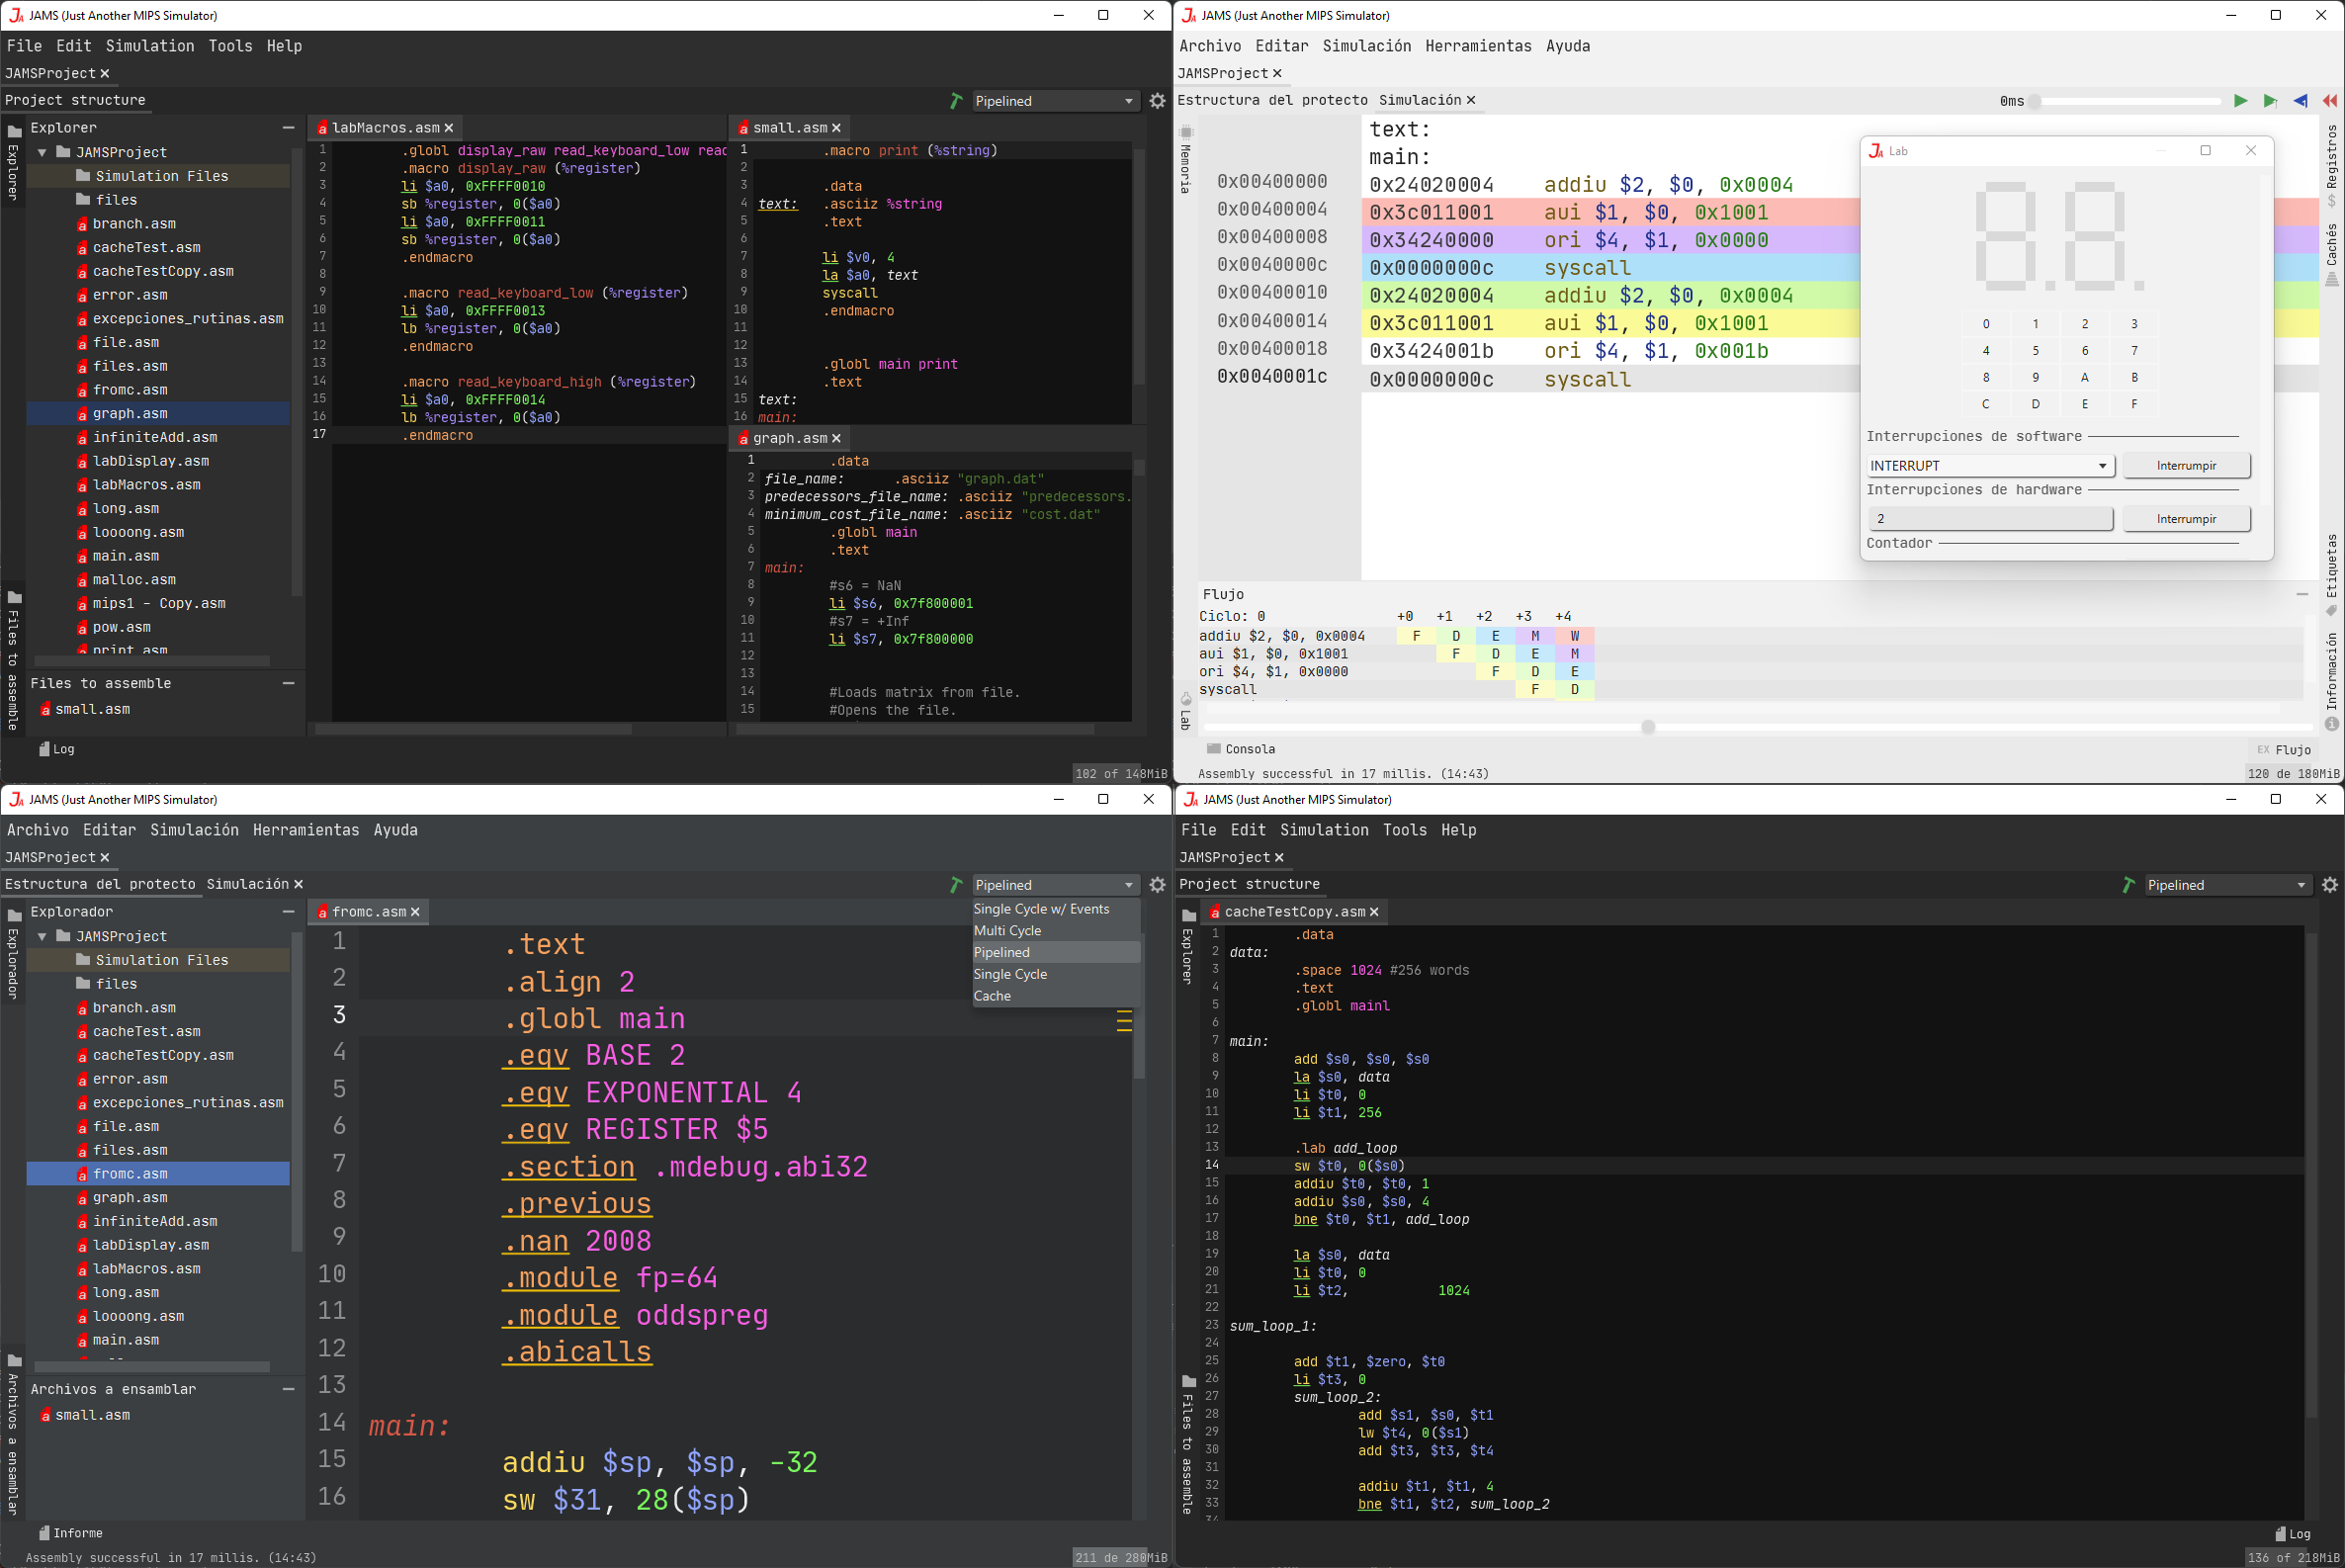
\includegraphics[width=0.8\textwidth]{images/introduction/jams-collage}
    \caption{Diferentes aspectos de \textit{JAMS}}
    \label{fig:jams-collage}
\end{figure}

\section{Descripción del problema}\label{sec:descripcion-del-problema}

Aunque tiene una arquitectura modular y muy flexible, \textit{JAMS}
no posee la capacidad de \textbf{vincular y desvincular}
componentes, lo cual impide que otros desarrolladores expandan sus capacidades.

Independientemente de la capacidad de carga de componentes,
una arquitectura \textbf{nunca es completamente modificable} hasta que
se creen componentes para su aplicación: es necesario
\textbf{desarrollar un componente} de prueba que cubra
todos los aspectos del entorno de desarrollo.

La \textit{NES} es una consola muy importante para la historia
del videojuego, con una gran comunidad de desarrolladores detrás
de ella.
Sorprendentemente, no existe ningún entorno que permita
\textbf{desarrollar, ensamblar y simular} videojuegos de manera sencilla.
Lo más cercano que se puede encontrar son componentes
para entornos de desarrollo generales con soporte básico de edición y
ensamblaje para el procesador \textit{MOS 6502}.


\section{Objetivos}\label{sec:objetivos}

El objetivo principal de este proyecto es proporcionar a \textit{JAMS}
un \textbf{sistema de vinculación de componentes}, que permita cargar
y descargar componentes de manera rápida y sencilla, permitiendo
a los desarrolladores expandir las capacidades del entorno de desarrollo.

También es necesario \textbf{estabilizar y mejorar}
la arquitectura de \textit{JAMS}, creando un componente
de prueba que cubra todos los aspectos del entorno de desarrollo.
Este componente introducirá \textbf{un editor, un ensamblador y un simulador}
enfocados en la arquitectura de la consola \textit{NES}, permitiendo
desarrollar videojuegos dentro de \textit{JAMS}.

A continuación se detallarán los diferentes objetivos parciales en los
que se ha descompuesto este objetivo principal.

\subsection{Desarrollo de un sistema de vinculación de componentes para \textit{JAMS}}
\label{subsec:desarrollo-de-un-sistema-de-vinculacion-de-componentes-para-jams}

Este es el \textbf{primer objetivo} que se debe superar en el transcurso de este
proyecto.
Para ello, se debe desarrollar un \textbf{vinculador de componentes} que permita
instalar y desinstalar componentes sin \textbf{tener que reiniciar la aplicación}.

\noexpand Este objetivo puede separarse en dos pasos:
\begin{itemize}
    \item Desarrollar el sistema base, que permita cargar código \textit{ByteCode}
    usando las librerías proporcionadas por el \textit{SDK} de \textit{Java}.
    \item Desarrollar un sistema de \textbf{proveedores}, permitiendo
    eliminar todos los elementos proporcionados por un componente
    cuando este sea desinstalado por el usuario.
\end{itemize}

\subsection{Desarrollo y mejora de tecnologías relacionadas con los componentes}
\label{subsec:desarrollo-y-mejora-de-tecnologias-relacionadas-con-los-componentes}

Este objetivo se centra en desarrollar y mejorar la tecnología de \textit{JAMS}
para permitir a los componentes modificar todos los aspectos del entorno de
desarrollo de una manera rápida y sencilla.

El desarrollo de estas tecnologías ha provocado la necesidad de
realizar modificaciones en el propio JAMS,
obteniéndose finalmente como resultado un código limpio y robusto.

\subsection{Creación de un entorno de desarrollo para la arquitectura \textit{NES}}
\label{subsec:creacion-de-un-entorno-de-desarrollo-para-la-arquitectura-mips32}

Para conseguir una librería robusta, se ha decidido desarrollar un componente
que proporcione a \textit{JAMS} un \textbf{editor}, un
\textbf{ensamblador} y un \textbf{simulador}
para la arquitectura de la consola \textit{NES}.
Este nuevo entorno de desarrollo debe proporcionarse \textbf{íntegramente}
mediante un componente que el usuario pueda instalar en la aplicación
principal.
Es decir, el código de \textit{JAMS} no debe proveer de ningún
tipo de tecnología específica para el desarrollo de la \textit{NES},
y tampoco debe existir en JAMS ninguna dependencia que requiera el uso de este componente.

Este entorno de desarrollo será muy similar al proporcionado
por \textit{JAMS} para la arquitectura \textit{MIPS32}, por lo que los
subobjetivos son muy parecidos:

\begin{itemize}
    \item Desarrollar un editor, un ensamblador y un simulador
    para la consola \textit{NES} usando la tecnología
    proporcionada por \textit{JAMS}.
    Estos tres componentes deben ser expandibles mediante otros componentes externos.
    \item Desarrollar diferentes herramientas que complementen las funcionalidades
    del editor, del ensamblador y del simulador.
\end{itemize}

A diferencia del entorno de desarrollo \textit{MIPS32}, del
  que ya dispone \emph{JAMS}, el entorno
de desarrollo para la \textit{NES} sí tiene como objetivo permitir crear
código válido que se pueda ejecutar en una consola real.


\section{Metodología}\label{sec:metodologia}

\begin{figure}[h]
    \centering
    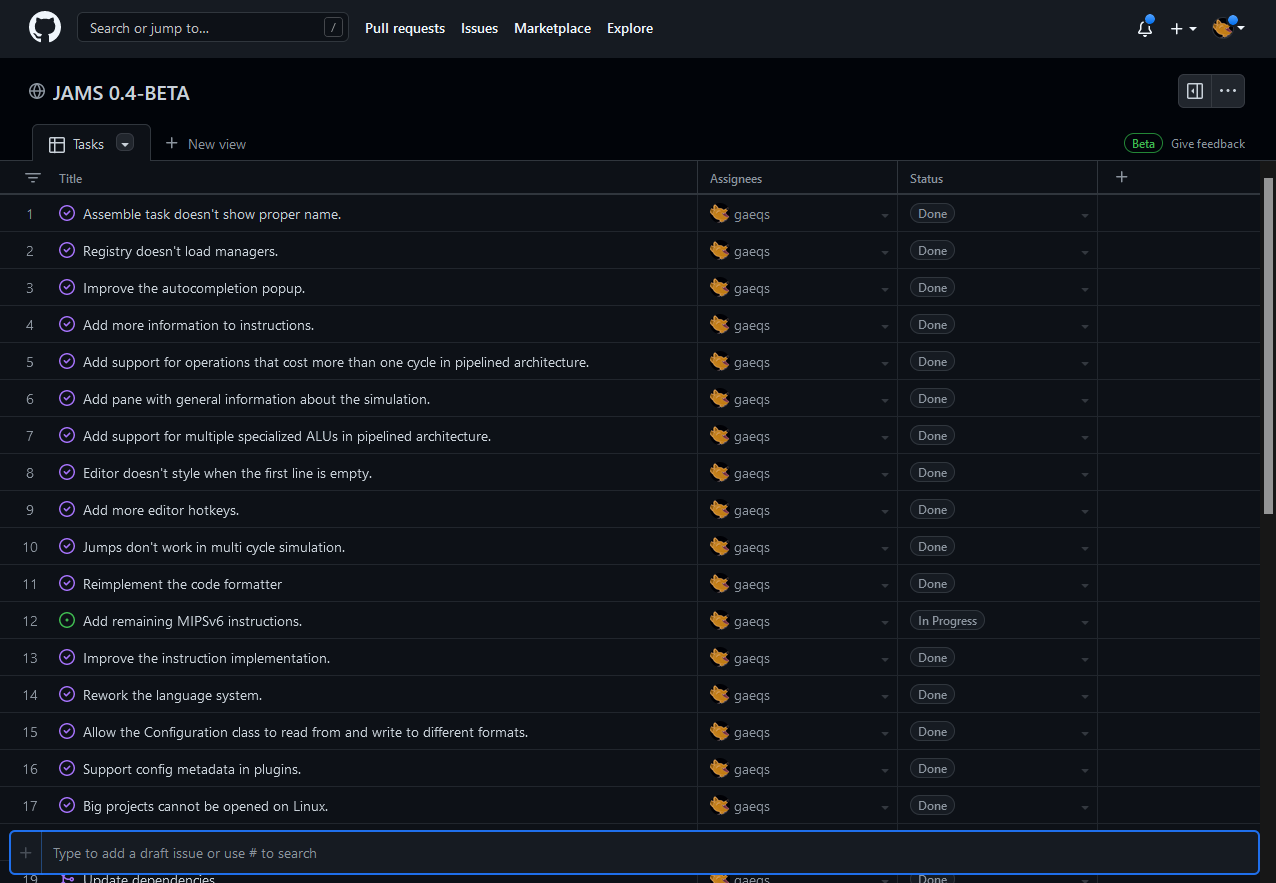
\includegraphics[width=\textwidth]{images/introduction/github}
    \caption{Proyecto de \textit{GitHub} para la versión 0.4-BETA}
    \label{fig:introduccion-github}
\end{figure}

Debido a que la aplicación principal es muy compleja,
es muy importante marcar una metodología que permita un
desarrollo consistente, eficiente y rápido.
\textit{JAMS} ha sido desarrollado mediante una \textbf{metodología ágil},
con \textit{sprints} donde se desarrollan una serie de características claves.
Todas las características se someten a varias iteraciones donde se modifican y mejoran hasta lograr un
buen resultado.
El desarrollo de \textit{JAMS} también ha seguido un desarrollo
basado en pruebas unitarias, permitiendo mantener la calidad del
código mientras la aplicación va evolucionando.

Toda la metodología ha sido implementada mediante
las herramientas proporcionadas por \textit{GitHub}.
Los estados de las características asignadas a un \textit{sprint}
se documentan mediante proyectos, como se observa en la figura \ref{fig:introduccion-github}.
Las acciones obligan a que las pruebas unitarias deban superarse
sin errores si se desea añadir una nueva característica a la rama principal.
Estas acciones también se emplean para generar los binarios
cuando se supera un \textit{sprint} y se lanza una
nueva versión de \textit{JAMS} .

El componente con el entorno de desarrollo \textit{NES}
también ha seguido esta filosofía, pero a menor escala, siendo el
tiempo entre cada versión \textit{alpha} mucho menor comparado
con la aplicación principal.

    \clearpage{\pagestyle{empty}\cleardoublepage}

    \chapter{Antecedentes}\label{ch:antecedentes}


\section{Antecedentes en los sistemas de componentes}
\label{sec:antecedentes-en-los-sistemas-de-componentes}

Los componentes son una parte \textbf{importante} de muchas aplicaciones
orientadas a los usuarios finales.
En esta sección se presentará algunas aplicaciones que permiten
la instalación de componentes:

\begin{itemize}
    \item \textbf{Navegadores web}: los navegadores web
    son las principales aplicaciones con complementos.
    Programas como \textit{Firefox} o \textit{Google Chrome}
    presentan una \textbf{tienda} donde el usuario puede instalar
    componentes con un solo clic.
    Estos componentes suelen estar desarrollados en \textit{JavaScript}
    o \textit{TypeScript}.
    \item \textbf{Entornos de desarrollo integrados}: los entornos de
    desarrollo más conocidos también tienen la capacidad de expandir
    sus herramientas mediante componentes.
    Estos componentes pueden introducir desde pequeños cambios
    a \textbf{tecnologías nuevas} a la aplicación, y suelen
    estar programados en el mismo lenguaje de programación
    que el entorno de desarrollo.
    Ejemplos de entornos de desarrollo con componentes
    son \textit{Intellij IDEA} y \textit{Eclipse},
    ambos con componentes desarrollados en \textit{Java}.
    \item \textbf{Videojuegos}: existe una gran variedad
    de videojuegos con posibilidad de expansión mediante
    componentes, llamados en este entorno \textit{\textbf{mods}}.
    Las librerías que proporcionan soporte para \textit{mods}
    pueden estar desarrolladas por los jugadores o venir
    integradas en el juego base.
    Un ejemplo de librerías desarrolladas por jugadores es
    \textit{Spigot} para \textit{Minecraft}, y un ejemplo
    de librerías integradas por los desarrolladores
    serían los videojuegos de \textit{Steam} con soporte
    para \textit{Steam Workshop}.
    \item \textbf{Aplicaciones en la nube}: existen
    algunas aplicaciones en la nube que permiten
    al usuario complementar su experiencia con diversos
    componentes desarrollados por terceros.
    Es el caso de \textit{Google Drive}, el cual permite
    instalar componentes para la visualización y
    edición de archivos.
    Este enfoque de los componentes es muy interesante,
    ya que es el \textbf{proveedor de la aplicación} el que
    instala el componente y no el usuario.
\end{itemize}


\section{Antecedentes en el desarrollo para la consola \textit{NES}}
\label{sec:antecedentes-en-el-desarrollo-para-la-consola-nes}

Existe una gran cantidad de herramientas para poder desarrollar
una aplicación o videojuego para la consola \textit{NES}.
Las principales son las \textbf{proporcionadas por \textit{Nintendo}}
en la década de los 80 a las desarrolladoras, pero estas
aplicaciones son muy antiguas y necesitan un kit de desarrollo
completo que solo \textit{Nintendo} puede proporcionar.
Las aplicaciones que se utilizan actualmente están
\textbf{desarrolladas por personas externas} a la compañía,
manteniendo vivo el desarrollo y uso de esta consola.

 Estas herramientas resuelven problemas muy concretos
presentes en el desarrollo de videojuegos, y ninguna
de ellas puede considerarse un entorno de desarrollo integrado.
Algunas de estas herramientas son las siguientes:

\begin{itemize}
    \item \textbf{Nestopia}: \textit{Nestopia} es uno de los emuladores
    para la consola \textit{NES} más importantes.
    Desarrollado en \textit{C++}, \textit{Nestopia} tiene soporte
    para más de 200 mapeadores y gran cantidad de periféricos.
    Nestopia está considerado uno de los emuladores más
    fieles que existen.
    \item \textbf{Asm6f}: ensamblador de código abierto
    para el código ensamblador 6052.
    \textit{Asm6f} permite ensamblar el código en
    \textbf{archivos \textit{INES 2.0}}
    que pueden utilizarse en emuladores, además
    de tener características especiales como soporte
    para instrucciones ilegales.
    \item \textbf{NEXXT}: \textit{NEXXT} es una pequeña
    aplicacion que permite editar los gráficos de los
    videojuegos de la \textit{NES}.
    La aplicación cuenta con funciones para recrear escenas
    mediante los \textit{tilesets} creados.
\end{itemize}
    \clearpage{\pagestyle{empty}\cleardoublepage}

    \chapter{Sistema de vinculación de componentes}\label{ch:sistema-de-vinculacion-de-componentes}

En este capítulo se abordará la creación de un sistema de
vinculación de componentes para \textit{JAMS}, empezando por
la estructura de un componente y terminando por la carga
del mismo dentro de \textit{JAMS}.

\section{Estructura de un componente}\label{sec:estructura-de-un-componente}

Los componentes, al igual que en muchas aplicaciones \textit{Java},
están conformados por un archivo \textit{jar} con el código que
se desea usar en la aplicación principal.
Más concretamente, un componente de \textit{JAMS} debe contener
dos elementos esenciales:
\begin{itemize}
    \item \textbf{Punto de entrada}: está conformado por una
    clase que extiende a $Plugin$.
    \textit{JAMS} crea una instancia de esta clase para
    poder ejecutar el código externo.
    \item \textbf{Archivo de metadatos}: confirmado por un archivo
    \textit{JSON}\cite{JSON} $plugin.json$ en la raíz del archivo \textit{jar}.
    Este archivo contiene los parámetros globales del componente,
    como pueden ser el \textbf{nombre}, la dirección del
    \textbf{punto de entrada}, la versión, los autores,
    o la descripción.
    Un ejemplo de archivo $plugin.json$ se puede observar en la
    figura \ref{fig:plugin-json}.
\end{itemize}


\begin{figure}[h]
    \centering
    \begin{lstlisting}[frame=single,label={lst:plugin-json}]
{
  "name": "NES4JAMS",
  "main": "io.github.gaeqs.nes4jams.NES4JAMS",
  "version": "0.1-ALPHA",
  "authors": [
    "Gael Rial Costas"
  ],
  "favicon": "/gui/icon/favicon.png",
  "description_node": "NES4JAMS_DESCRIPTION"
}
    \end{lstlisting}
    \caption{Ejemplo de archivo $plugin.json$}
    \label{fig:plugin-json}
\end{figure}

\subsection{Dependencias}\label{subsec:dependencias}

Un componente puede depender de otro componente.
Para proporcionar una inicialización de los componentes
correcta se proporcionan los parámetros $dependencies$
y $soft\_dependencies$, los cuales se pueden utilizar en
el archivo $plugin.json$.
Todos los componentes cuyo nombre esté dentro de una de estas
listas será inicializado antes.
Si no se encuentra ningún componente que tenga el nombre
de algún valor de $dependencies$, el componente no
se inicializará, lanzando una excepción.
Cabe destacar que dos componentes no pueden conformar
una \textbf{dependencia cíclica}.

\subsection{Puntos de entrada}\label{subsec:puntos-de-entrada}

Como ya se ha mencionado, un punto de entrada está conformado
por una \textbf{clase que extiende a $Plugin$}.
El desarrollador puede extender dos métodos definidos por esta clase:
$onEnable$ y $onEnable$, los cuales serán llamados cuando el
componente es vinculado o desvinculado de la aplicación principal.
Un ejemplo de punto de entrada se puede observar en la figura \ref{fig:entry-point}.

\begin{figure}[h]
    \centering
    \begin{lstlisting}[frame=single,label={lst:entry-point},language=Kotlin]
class MyPlugin : Plugin() {

    override fun onEnable() {
        println("My plugin has been enabled!")
        if (JamsApplication.isLoaded()) {
            loadApplicationData()
        }
    }

    override fun onDisable() {
        println("My plugin has been disabled!")
    }

    @Listener
    fun onApplicationLoad(event: JAMSApplicationPostInitEvent)
        = loadApplicationData()

    private fun loadApplicationData() {
        println("Now I can access the JavaFX application!")
    }

}
    \end{lstlisting}
    \caption{Ejemplo de punto de entrada de un componente desarrollado en \textit{Kotlin}}
    \label{fig:entry-point}
\end{figure}

 El punto de entrada puede ser inicializado en diferentes
etapas del proyecto: el componente será cargado antes del contexto
de \textit{JavaFX} si este ya estaba instalado en la aplicación
cuando esta es lanzada.
Es por eso que el desarrollador debe \textbf{comprobar si el contexto ha sido creado}
antes de añadir o modificar nuevos elementos.
Si el contexto aún no ha sido creado, los componentes podrán
usar el evento $JAMSApplicationPostInitEvent$ para ejecutar
código cuando este sea inicializado.
Este sistema de eventos se verá en profundidad en esta memoria más adelante.


\section{Vinculación de un componente}\label{sec:vinculacion-de-un-componente}

Un componente puede ser vinculado de dos maneras diferentes:
cuando el usuario \textbf{instala el componente} desde la aplicación
y cuando la \textbf{aplicación principal es inicializada} y el componente
está ya instalado.
La vinculación de componentes difiere en varios aspectos en estas
dos situaciones: cuando el componente es instalado, \textit{JAMS}
comprueba si \textbf{todas sus dependencias fuertes están presentes}.
Si esto no se cumple, el componente no puede ser instalado.
Cuando la aplicación principal es inicializada esta debe vincular
una cantidad no definida de componentes.
Es por ello que debe generar un \textbf{grafo de dependencias}
antes de inicializar los componentes.

\section{Desvinculación de un componente}\label{sec:desvinculacion-de-un-componente}

Un componente es desvinculado de la aplicación principal
cuando el usuario \textbf{desinstala el componente} desde
la aplicación o cuando la \textbf{aplicación principal es cerrada}.
De la misma manera que en la vinculación, el proceso de
desvinculación \textbf{difiere} en ambas circunstancias.
Para que un componente sea desinstalado, el usuario
debe desinstalar previamente \textbf{todos los componentes
que dependen} del componente a desinstalar.
Solo cuando no exista ningún componente dependiente
es cuando se puede desinstalar el componente deseado.
Cuando la aplicación principal es cerrada
\textbf{no se desvincula ningún componente},
únicamente se llama al método $onDisable$, dejando
el proceso de desvinculación a la \textit{JVM}.

\section{Interfaz de usuario}\label{sec:interfaz-de-usuario}

Los usuarios pueden instalar o desinstalar componentes
desde la \textbf{ventana de configuración}.
En esta interfaz se mostrará la lista de componentes
que están instalados junto con el nombre, la versión
y la descripción de estos.

\begin{figure}[h]
    \centering
    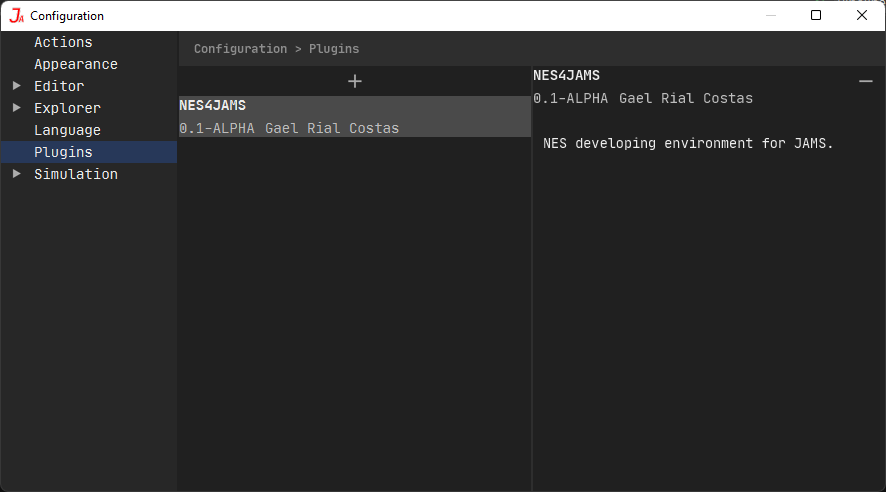
\includegraphics[width=\textwidth]{images/componentes/plugin-ui}
    \caption{Sección de componentes en la configuración}
    \label{fig:plugin-ui}
\end{figure}
    \clearpage{\pagestyle{empty}\cleardoublepage}

    \chapter{Entorno de desarrollo \textit{NES}}\label{ch:entorno-de-desarrollo-nes}

En este capítulo se abordará el análisis del desarrollo de \textit{NES4JAMS},
un componente que aporta a \textit{JAMS} un entorno de desarrollo
integrado para la creación de videojuegos para la consola
\textit{NES}.
Gracias a la arquitectura de \textit{JAMS}, este componente
aprovechará muchas de las características creadas
para el entorno de desarrollo \textit{MIPS32} presente
por defecto en la aplicación.
Este entorno de desarrollo consistirá en un editor
de texto, un ensamblador y un simulador.


\section{Creación de un proyecto}\label{sec:creacion-de-un-proyecto}

\begin{figure}[h]
    \centering
    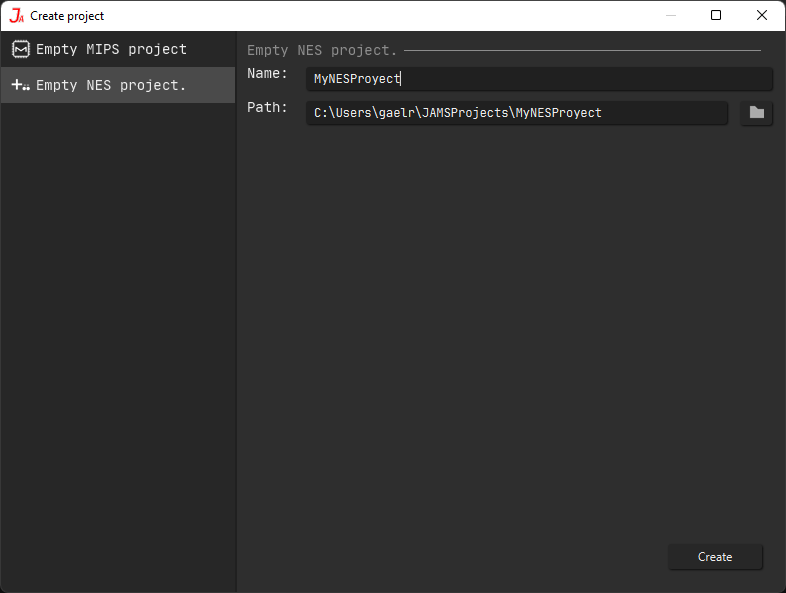
\includegraphics[width=0.85\textwidth]{images/nes/nes-project-creation}
    %% Óscar: he cambiado el width de 0.8 a 0.85 para que no se quede
    %% una línea sola al final, que queda fatal.
    \caption{Creación de un proyecto \textit{NES}}
    \label{fig:nes-project-creation}
\end{figure}

\textit{NES4JAMS} añade a \emph{JAMS} un nuevo tipo de proyecto
que incorpora todas las herramientas para el desarrollo
de videojuegos para \textit{NES}.
Los usuarios podrán crear nuevos proyectos de este tipo
desde el menú de creación de proyectos.
Como los proyectos de \textit{NES} están destinados
a una consola muy específica, el usuario solo debe
especificar \textbf{el nombre y la localización del proyecto},
como se puede observar en la figura \ref{fig:nes-project-creation}.

Una vez creado el proyecto, \textit{JAMS} mostrará una ventana
principal muy similar a la de los proyectos \textit{MIPS32}.


\section{Editor}\label{sec:editor}

Los desarrolladores de videojuegos para \textit{NES} trabajan con
dos tipos de archivos principales: los archivos \textit{asm}
para el código y los archivos \textit{pcx} para los gráficos.
\textit{NES4JAMS} permite al usuario editar los dos tipos de archivo
de manera sencilla.

Cuando el usuario desea editar uno de estos archivos,
debe seleccionarlo en la herramienta \textbf{explorador}.
Esta herramienta muestra una representación de la
estructura del proyecto en forma de árbol.
El usuario puede expandir y contraer carpetas, así como crear,
borrar y mover archivos.
Si el usuario hace doble clic sobre un archivo editable, este se abrirá
en el editor.
Dependiendo del tipo de archivo, el editor será diferente,
como se puede observar en la figura \ref{fig:nes-editor}.

\begin{figure}[h]
    \centering
    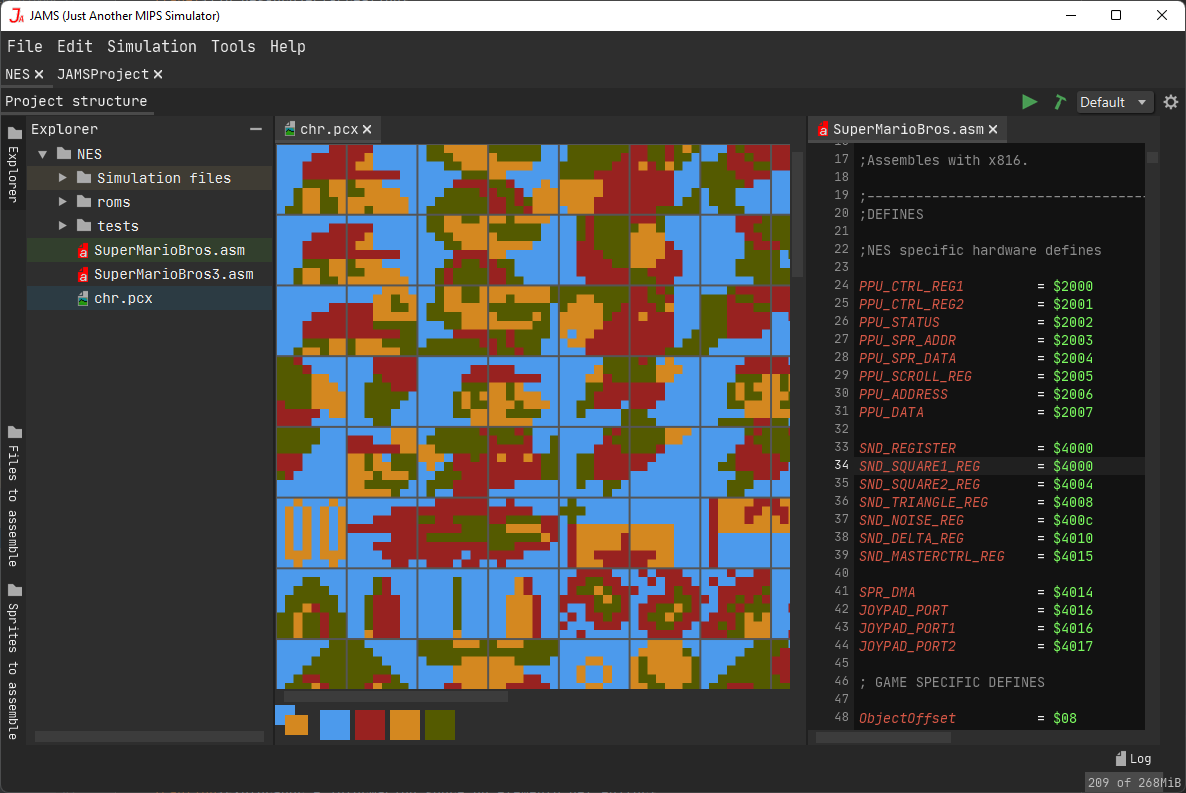
\includegraphics[width=0.8\textwidth]{images/nes/nes-editor}
    \caption{Editor de código y de gráficos junto con el explorador}
    \label{fig:nes-editor}
\end{figure}

El menú contextual del explorador presenta varias acciones que
pueden ejecutarse sobre las carpetas y los archivos
del proyecto.
Una de las opciones más particulares es la opción de añadir o eliminar
archivos de código o de gráficos del ensamblador.
Al ser \textit{JAMS} un entorno de desarrollo basado en \textbf{proyectos},
es necesario proporcionar una manera de incluir o excluir archivos del
videojuego resultante.
Con este sistema tan sencillo, el usuario podrá elegir qué archivos es preciso ensamblar.
Estos archivos para ensamblar estarán marcados en \textbf{verde} en el explorador,
y aparecerán en orden en los nodos \textbf{Archivos para ensamblar} y
\textbf{\textit{Sprites} para ensamblar}.
Cabe destacar que, como se verá más adelante, el orden de ensamblaje
importa, por lo que esta herramienta permite ordenar los ficheros de una manera sencilla.

Una vez el usuario abra un archivo, su editor aparecerá en la herramienta
principal de la sección: \textbf{el visualizador de archivos}.
\textit{NES4JAMS} añade dos editores nuevos a \textit{JAMS}:
el editor de código \textit{MOS 6502} y el editor de gráficos \textit{PCX}.

\subsection{Editor de código}\label{subsec:editor-de-codigo}

El editor de código usa el sistema de indexación desarrollado
en la capa base de \textit{JAMS}, por lo que este editor también
puede considerarse un \textbf{editor de texto inteligente}:
el editor convierte el texto puro en los componentes ensamblador
representados, pudiendo así aportar ayudas al usuario.
El editor también tiene conocimiento de las referencias y el alcance de
todas las etiquetas y macros, tanto en el propio archivo editado
como en el resto de archivos fuente del proyecto.
El editor también incorpora un \textbf{autocompletador}.
Esta herramienta ayuda al usuario cuando escribe código
aportando sugerencias de autocompletación, como se puede
observar en la figura \ref{fig:nes-autocompletion}.

\begin{figure}[h]
    \centering
    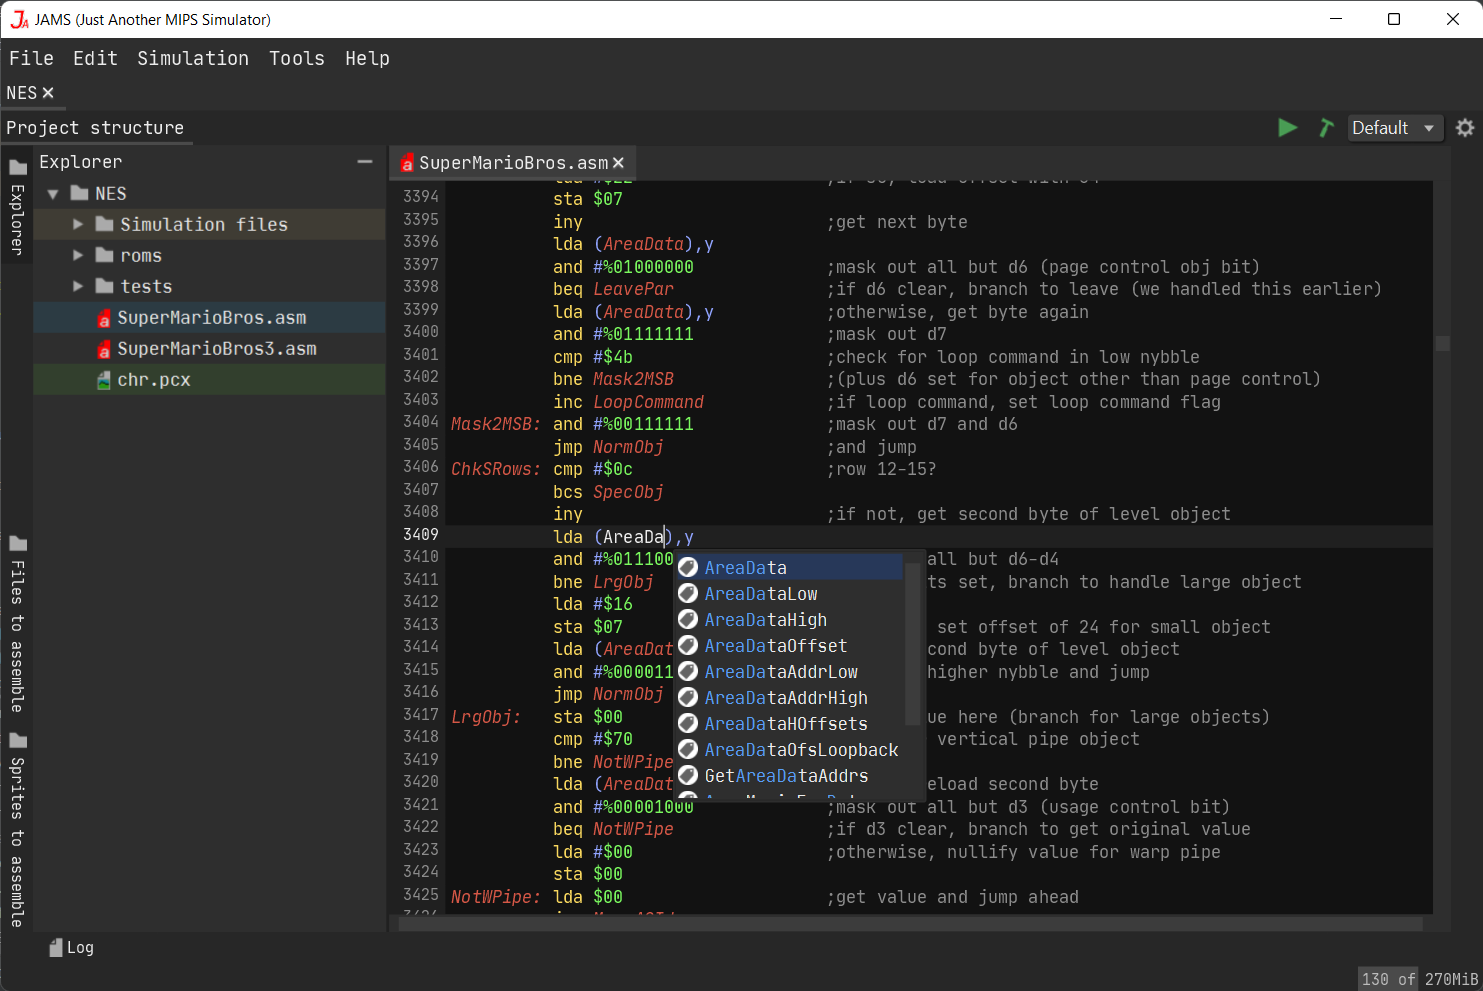
\includegraphics[width=0.8\textwidth]{images/nes/nes-autocompletion}
    \caption{Autocompletador ayudando al usuario}
    \label{fig:nes-autocompletion}
\end{figure}

\subsection{Editor de gráficos}\label{subsec:editor-de-graficos}

\textit{PCX} es un formato de imagen desarrollado
en el año 1985 que cuenta con una codificación \textit{run-length}.
Actualmente, el formato ha caído en desuso, pero sus propiedades
lo hacen un \textbf{gran candidato} para almacenar gráficos
de la \textit{NES} antes de ser ensamblados.
Esto se debe a su capacidad de codificar los colores mediante
una \textit{paleta} de una manera sencilla.
Al almacenar los valores de los píxeles como índices y no
como colores, el formato \textit{PCX} se convierte en un
candidato ideal para gráficos dependientes de una paleta
externa, como es el caso de los gráficos de una \textit{NES}.

El editor de archivos \textit{PCX} permite modificar los
gráficos del videojuego de una manera rápida y sencilla.
Este editor está pensado exclusivamente para gráficos
de \textit{NES} (patrones a los que se les aplica una
paleta de cuatro colores), por lo que cada pixel solo puede tomar
cuatro valores diferentes.
El color final se buscará en la paleta seleccionada.
El usuario puede cambiar el color de cada elemento de la
paleta utilizando el botón central del ratón sobre
la entrada seleccionada.
Por motivos de accesibilidad, el usuario también puede
cambiar el color empleando el botón principal del
ratón mientras mantiene pulsada la tecla $Ctrl$.

Cabe destacar que, aunque este editor permite editar
archivos \textit{PCX} de cualquier tamaño, la consola
leerá el archivo como si tuviera un ancho de 128 píxeles.
Esto es debido a que las tablas donde se guardan los gráficos
en la consola tienen un tamaño de 16x16 patrones
de 8x8 píxeles cada uno.
Si se ensambla un archivo \textit{PCX} con otro ancho,
lo más probable es que los gráficos se conviertan en
\textbf{ruido}.
Los archivo\newODR{s} \textit{PCX} creados por \textit{NES4JAMS}
siempre tienen el tamaño de una tabla de patrones,
es decir, de 128x128 píxeles.

\begin{figure}[h]
    \centering
    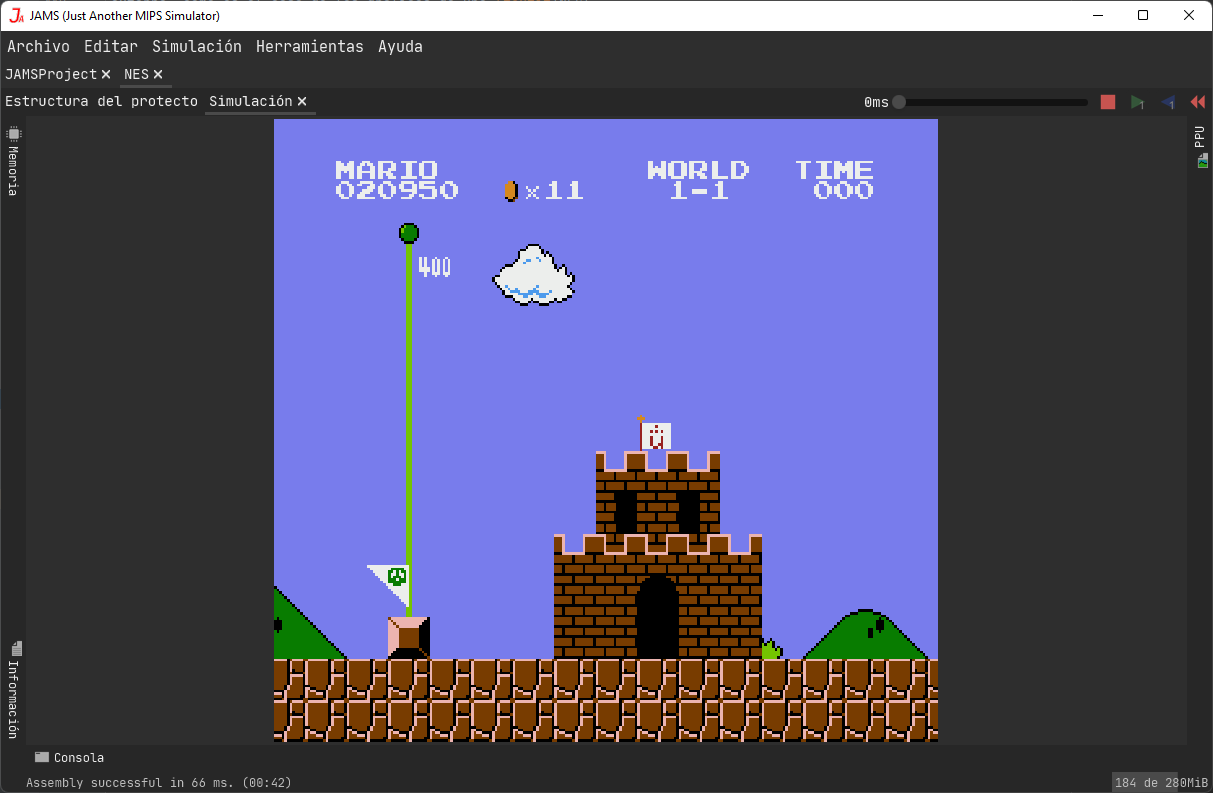
\includegraphics[width=0.8\textwidth]{images/nes/nes-graphics-change}
    \caption{\textit{Super Mario Bros.} con los gráficos modificados}
    \label{fig:nes-graphics-change}
\end{figure}

\subsection{Archivos iNES}\label{subsec:archivos-nes}

El formato \textit{iNES} es el formato de archivo más utilizado
para almacenar videojuegos para la consola \textit{NES}.
Este formato comienza con una cabecera con los datos que suelen
estar codificados en el propio cartucho, como puede ser el modo
espejo, el controlador de memoria o la región.
La cabecera también contiene el tamaño de la región del
programa (\textit{PGR}) y la región de gráficos (\textit{CHR})
que van detrás de ella.

\textit{NES4JAMS} es capaz de \textbf{cargar y generar} archivos
\textit{iNES} de manera nativa.
Al abrir un archivo \textit{iNES}, \textit{NES4JAMS} mostrará
el editor mostrado en la figura \ref{fig:nes-ines-editor}.

\begin{figure}[h]
    \centering
    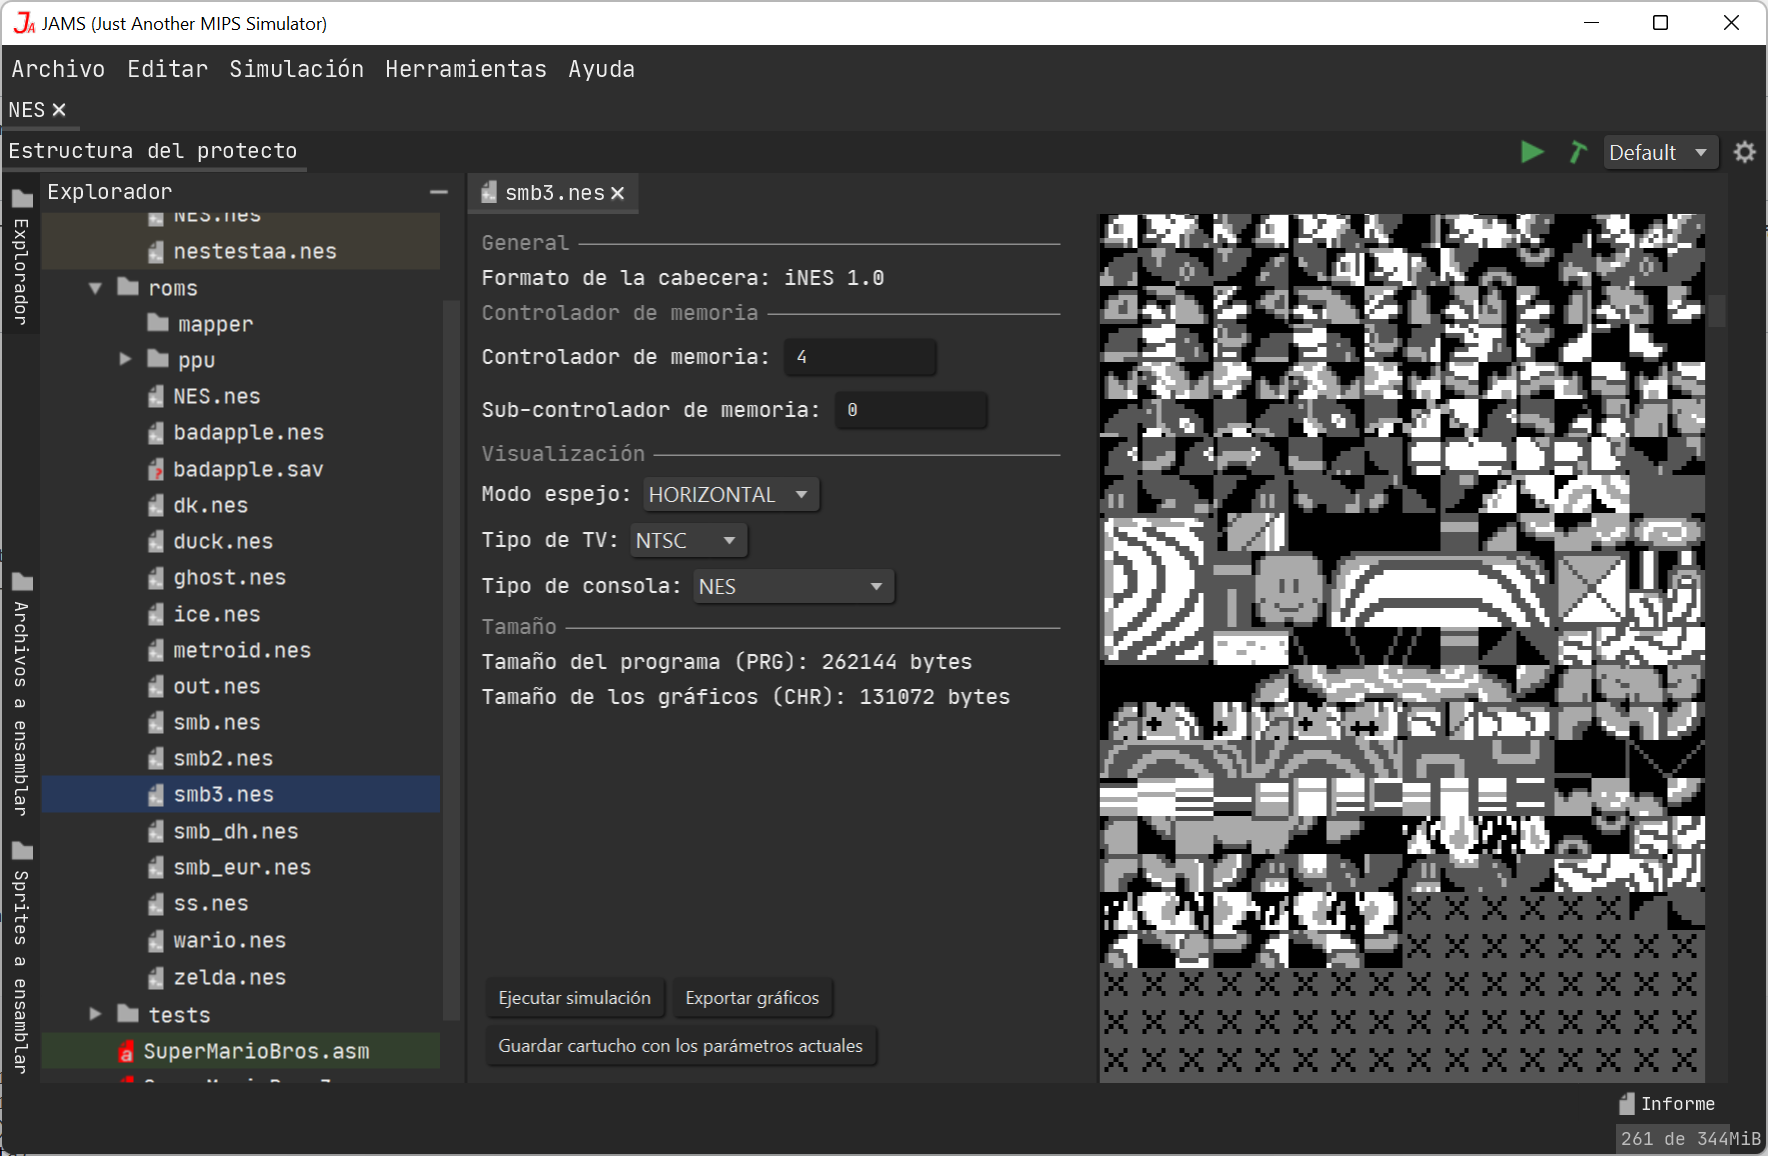
\includegraphics[width=0.8\textwidth]{images/nes/nes-ines-editor}
    \caption{Archivo \textit{iNES} en el editor}
    \label{fig:nes-ines-editor}
\end{figure}

En este editor el usuario podrá ejecutar una simulación
para el videojuego seleccionado, permitiéndole \textbf{modificar}
parámetros de cabecera.
El usuario también tiene la opción de \textbf{exportar las tablas
de patrones} del cartucho en un archivo \textit{PCX}.
Se puede observar una previsualización de estas tablas en la parte derecha del editor.
Por último, el editor ofrece la opción de \textbf{guardar una copia}
del videojuego con los parámetros modificados.

\subsection{Configuraciones}\label{subsec:configuraciones}

\begin{figure}[h]
    \centering
    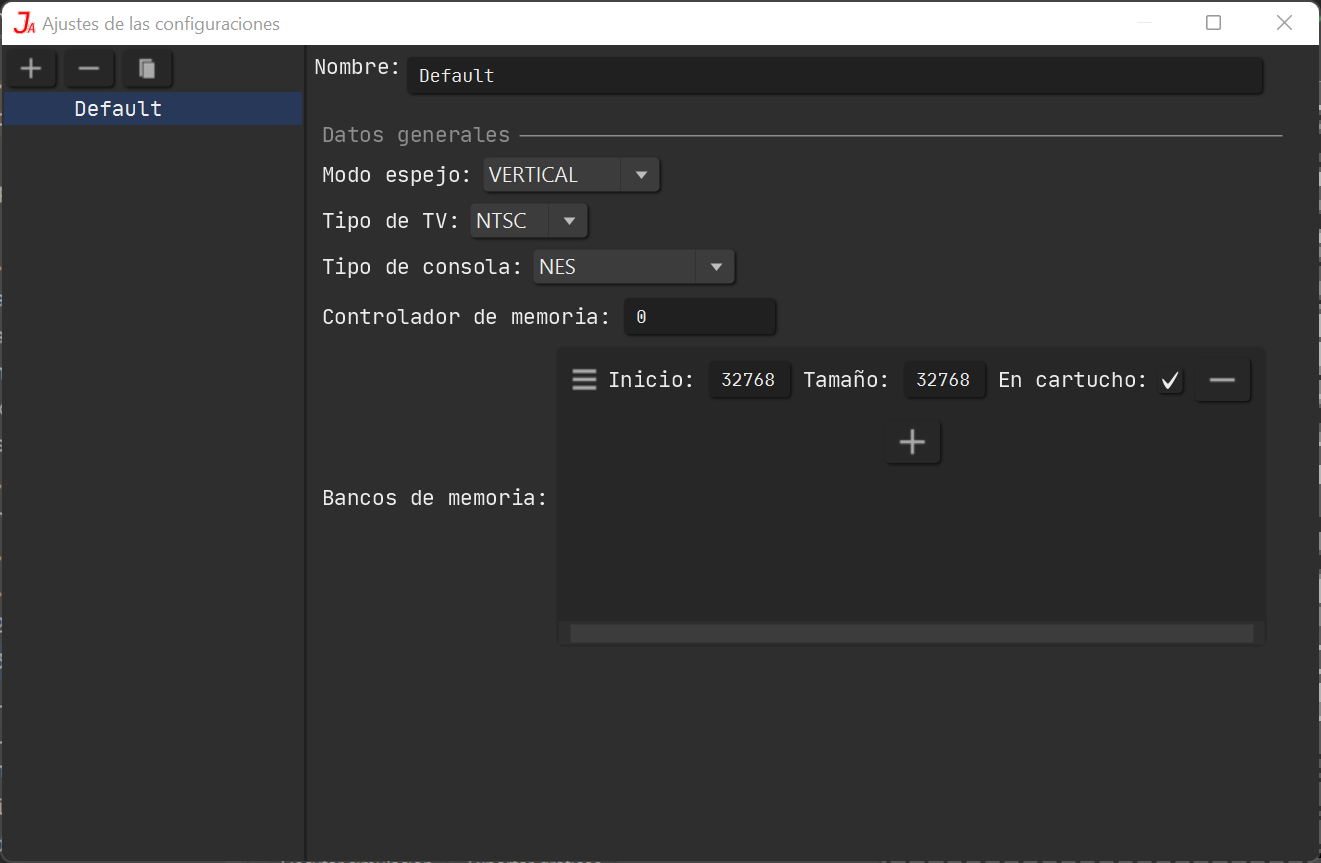
\includegraphics[width=0.8\textwidth]{images/nes/nes-configurations}
    \caption{Menú de configuraciones\note{Insisto: tienes que
        referenciar todas las figuras en el texto, y esta no lo está}}
    \label{fig:nes-configurations}
\end{figure}

Igual que en el entorno de desarrollo para \textit{MIPS32},
el entorno de desarrollo \textit{NES} permite ensamblar
el programa con diferentes \textbf{configuraciones}.
Estas configuraciones definen los \textbf{parámetros de la cabecera}
del archivo \textit{iNES} resultante y los \textbf{bancos de memoria}
presentes en el cartucho.

Los bancos de memoria están definidos por una \textbf{dirección de inicio}
y un \textbf{tamaño} en bytes.
De manera muy similar a las directivas \textit{.text}
y \textit{.data} de \textit{MIPS32}, el desarrollador podrá
alternar entre bancos de memoria usando la directiva \textit{.bank}.

\textit{NES4JAMS} también incorpora una opción que impide copiar un
banco de memoria en el cartucho.
Esta funcionalidad es muy importante para algunos videojuegos
avanzados, ya que les permite utilizar un banco de memoria como
una representación de una \textbf{memoria RAM} adicional
dentro del cartucho.

La interfaz usada para modificar estas configuraciones puede observarse
en la figura \ref{fig:nes-configurations}.


\section{Ensamblador \textit{MOS 6502}}\label{sec:ensamblador}

El ensamblador para el procesador \textit{MOS 6502} se utiliza
para convertir los proyectos en archivos \textit{iNES}.
Este ensamblador soporta características avanzadas empleadas
comúnmente al programar, como las macros,
las etiquetas globales o las referencias relativas.
El código fuente de un proyecto se ensambla en \textbf{cuatro pasos}:
descubrimiento, expansión, asignación de direcciones y asignación de valores.
Estos son los mismos pasos que utiliza el ensamblador para \textit{MIPS32},
y es que el del \textit{MOS 6502} presenta \textbf{la misma arquitectura}
que el incluido por defecto en \textit{JAMS}.

\subsection{Descubrimiento}\label{subsec:descubrimiento}

En este paso el texto del proyecto se \textbf{descompone en sus primitivas},
permitiendo al ensamblador descubrir los diferentes componentes de cada línea.
Al final de este paso, las etiquetas globales y las etiquetas del archivo
(etiquetas no definidas dentro de una macro) \textbf{son registradas sin
ningún valor asignado}.
También se registran las macros de cada archivo.
El identificador de una macro es definido por su nombre concatenado
al número de parámetros que necesitan.
Este procedimiento se realiza para dar soporte a la sobrecarga de macros.
En el caso de la macro $print$, su identificador sería
$print-1$.

Cabe destacar que, a diferencia del ensamblador para \textit{MIPS32},
las etiquetas pueden hacer referencia a una dirección de memoria
o a una \textbf{equivalencia}.
Estas equivalencias relacionan una etiqueta con una expresión matemática
que a la vez puede hacer uso de otras etiquetas para calcular su valor.

\subsection{Expansión}\label{subsec:expansion}

En este paso, se invocan las llamadas a macro,
insertando el código de la macro en la posición de la llamada.
Este código efectúa el primer paso del ensamblaje mientras es añadido.
Al insertarse justo después de la llamada, el código de la macro
también será expandido.

\subsubsection{Alcance}\label{subsubsec:alcance}

Las etiquetas y macros que están dentro de una macro
\textbf{tienen un alcance diferente al del archivo}.
Si la macro es global, el alcance es considerado hijo del alcance global
y no podrá acceder a las etiquetas del archivo que lo invoca.
Si la macro es local, el alcance es considerado hijo del alcance del archivo.

Cuando un alcance es hijo de otro alcance,
\textbf{el hijo podrá acceder a las etiquetas y macros de su padre}.
El hijo también podrá definir nuevas etiquetas y macros con el mismo
identificador que una etiqueta o macro de su padre.
Aunque este comportamiento está permitido, \textbf{el hijo solo podrá acceder
al elemento que él define}.
Esta funcionalidad es llamada \textbf{ocultamiento o \textit{shadowing}}.

\subsection{Asignación de direcciones}\label{subsec:asignacion-de-direcciones}

Una vez el ensamblador haya expandido las macros,
se asignan las direcciones de todas las instrucciones,
etiquetas y directivas que lo requieran.
Estas direcciones se asignan de manera secuencial.
Existen directivas que pueden modificar el flujo de la asignación,
como es el caso de la directiva $.bank$ anteriormente mencionada.

\subsection{Asignación de valores}\label{subsec:asignacion-de-valores}

Como paso final, el ensamblador insertará en memoria los valores
que representan las directivas e instrucciones.
Es en este paso donde se resuelven los valores de las equivalencias.

\subsection{Empaquetamiento}\label{subsec:empaquetamiento}

Como paso adicional fuera del ensamblador, los datos resultantes
en los bancos de memoria son empaquetados en un archivo \textit{iNES}.
Este archivo junta la cabecera especificada en la configuración seleccionada
por el usuario, los bancos de memoria especificados como memoria
\textit{ROM} y los gráficos traducidos a tablas de patrones.
Este archivo está situado en los archivos del simulador, lo que
permite que el desarrollador pueda distribuir su videojuego
y utilizarlo en otros emuladores.

\subsection{Características avanzadas}\label{subsec:características-avanzadas}

El ensamblador permite el uso de técnicas avanzadas en
el desarrollo de aplicaciones en lenguaje ensamblador, como
las que se detallan a continuación.

\begin{itemize}
    \item \textbf{Referencias relativas}: una directiva o instrucción puede \textbf{referenciar a una etiqueta de manera
    relativa} con las referencias especiales $+$ y $-$.
    La referencia $+$ hace referencia a la etiqueta siguiente.
    La referencia $-$ hace referencia a la etiqueta anterior.
    Las referencias relativas \textbf{solo pueden hacer referencia
    a etiquetas del mismo alcance}.
    No pueden hacer referencia a etiquetas de un alcance mayor.
    \item \textbf{Macros anidadas}: una macro puede ser definida dentro de otra macro.
    Esto es conocido como una \textbf{macro anidada}.
    Una macro anidada solo podrá ser accedida en el alcance de la macro
    en la que está declarada.
    \item \textbf{Expresiones}: las expresiones son la característica más avanzada
    presente en el ensamblador, y permite deducir el valor
    de una instrucción o directiva mediante una \textbf{expresión matemática}
    que puede usar etiquetas como parámetros.
    Los usuarios pueden emplear una gran variedad de operaciones
    en las expresiones, como son la suma, la resta, la multiplicación,
    la división y las operaciones lógicas a nivel de bit.
    También existen operaciones \textbf{unarias}, como son
    la conversión de un número en byte o palabra,
    la negación a nivel de bit o la selección del
    primer o segundo byte de una palabra.
    Estas expresiones se utilizan de manera directa en las
    instrucciones y directivas, como se observa en
    la figura \ref{fig:nes-expressions}.
\end{itemize}

\begin{figure}[h]
    \centering
    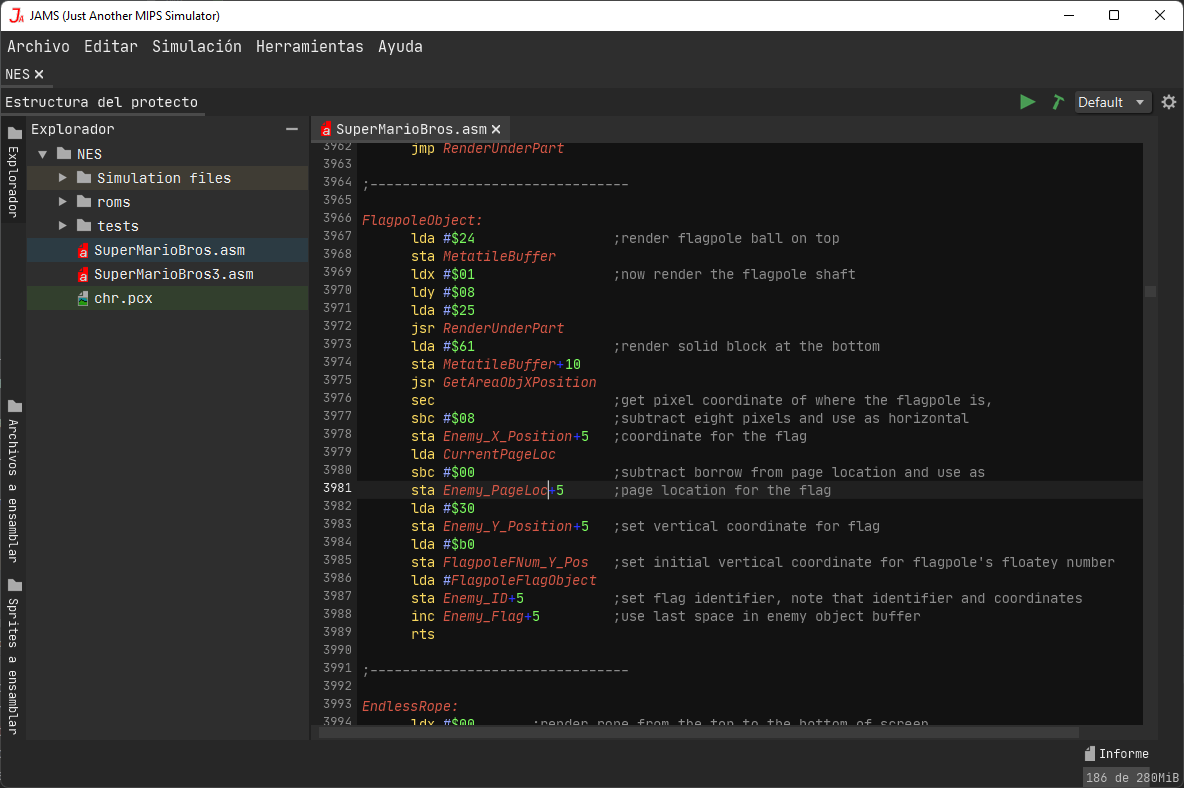
\includegraphics[width=0.8\textwidth]{images/nes/nes-expressions}
    \caption{Expresiones con sumas usadas en instrucciones}
    \label{fig:nes-expressions}
\end{figure}

\subsection{Detalles finales}\label{subsec:detalles-finales}

A diferencia del ensamblador para \textit{MIPS32},
este ensamblador no es muy personalizable.
Esto es debido a que \textit{NES4JAMS} pretende
ser un entorno de desarrollo de videojuegos para la \textit{NES}
que puedan ejecutarse en \textbf{consolas reales}.
\textit{NES4JAMS} da soporte para todas las
\textbf{instrucciones legales} presentes en la consola,
por lo que no es factible dar soporte para instrucciones
de terceros.


\section{Simulador}\label{sec:simulador}

Un simulador es una pieza de \textit{software} que imita el
comportamiento de un dispositivo.
\textit{NES4JAMS} introduce un simulador de la arquitectura
de la consola \textit{NES} que permite jugar y depurar
una gran variedad de videojuegos.

El simulador está principalmente compuesto por cinco partes:
la unidad central de procesamiento
(\textit{Central Processing Unit} o \textit{CPU}),
la unidad de procesamiento de imágenes
(\textit{Picture Processing Unit} o \textit{PPU}),
la unidad de procesamiento de audio
(\textit{Audio Processing Unit} o \textit{APU}),
el bus de datos y el controlador de memoria o \textit{mapper}.
El simulador simula el comportamiento de todos los componentes
en cada \textbf{ciclo de reloj}.

\subsection{Estructura del simulador}\label{subsec:estructura-del-simulador}

El nodo principal del simulador para la consola \emph{NES} no
es un visualizador de instrucciones, sino una herramienta que
simula la \textit{salida de vídeo} de la consola y que puede
observarse en la figura \ref{fig:nes-video}.

\begin{figure}[h]
    \centering
    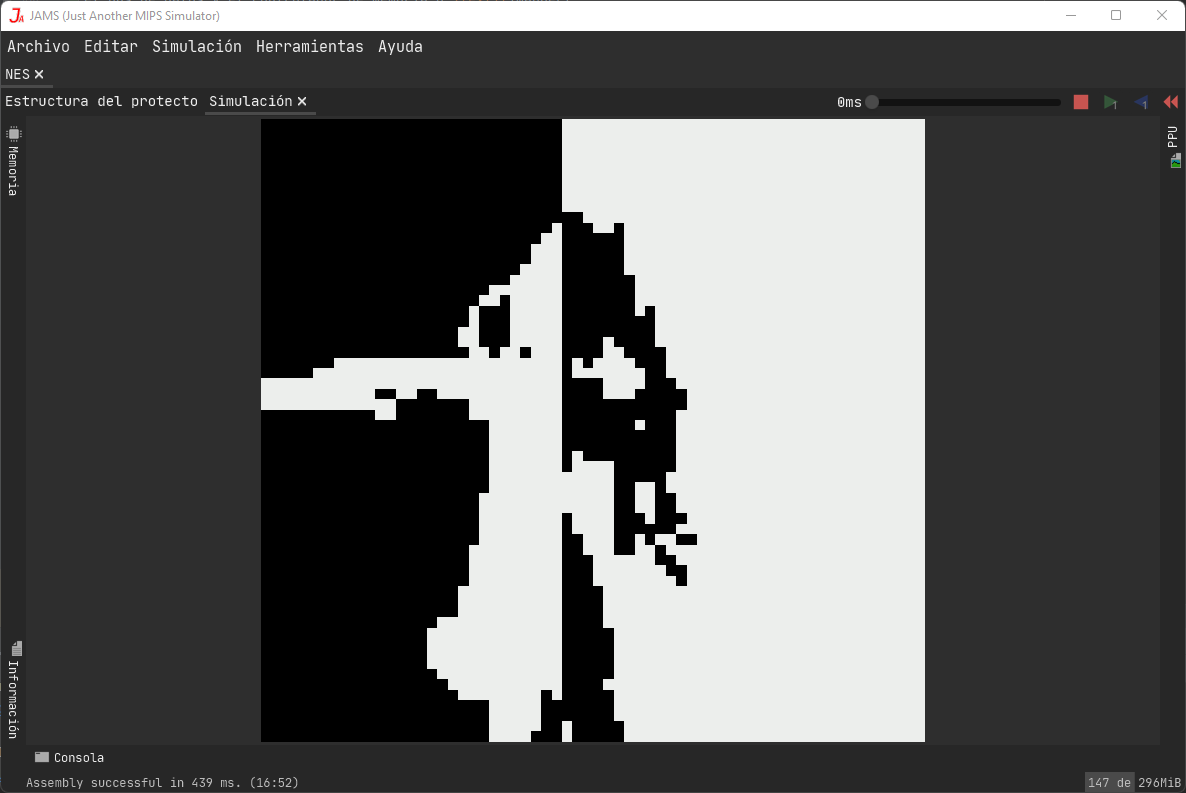
\includegraphics[width=0.8\textwidth]{images/nes/nes-video}
    \caption{Simulador reproduciendo una versión de \textit{Bad Apple!} para la \textit{NES}}
    \label{fig:nes-video}
\end{figure}

A diferencia de los cauces gráficos actuales, la \textit{NES}
compone la imagen de salida generando \textbf{un pixel} cada
ocho ciclos de reloj de la \textit{PPU}.
Este comportamiento, junto con otras características como
la generación de interrupciones de la unidad central
por parte de la propia \textit{PPU}, hace imposible usar
herramientas de renderizado avanzadas como las proporcionadas
por librerías como \textit{Vulkan} u \textit{OpenGL}.

La única manera de renderizar la salida de vídeo de la \textit{NES}
es generando la imagen en el \textbf{mismo hilo de ejecución}
utilizado por la \textit{CPU}.
De esta manera, la \textit{PPU} ejecuta una cantidad de ciclos
determinada por la región por cada ciclo de \textit{CPU}.

\textit{JavaFX} no está optimizada para modificar imágenes en movimiento.
La herramienta de vídeo emplea una versión \textbf{muy modificada}
de las imágenes proporcionadas por la librería,
permitiendo así modificar una imagen muchas veces por segundo
de manera constante.

Esta salida de vídeo se complementa con dos herramientas principales:
la herramienta \textit{memoria} y la herramienta \textit{PPU}.
Existen otras herramientas secundarias, como la \textit{consola}, que permite
visualizar el resultado de la simulación cuando se para, o
la \textit{información}, que permite visualizar el número de imágenes por segundo
mostradas en la salida de vídeo.

\subsection{Memoria}\label{subsec:memoria}

La memoria de la \textit{NES} puede separarse en \textbf{tres secciones}:
la memoria \textit{RAM}, la memoria del cartucho y la memoria \textit{VRAM}.
La memoria del cartucho está dividida en dos secciones:
la memoria del programa (\textit{PRG}), donde se guardan
las instrucciones del videojuego,
y la memoria de los gráficos (\textit{CHR}), donde se guardan
las tablas de patrones.
A su vez, la memoria \textit{VRAM} o \textit{RAM} de la \textit{PPU}
se divide también en dos secciones:
las tablas de nombres y las paletas de colores.

La consola presenta \textbf{dos buses de datos}:
el bus de datos de la \textit{CPU}
y el bus de datos de \textit{PPU}.
El bus de datos de la \textit{CPU} permite a
este acceder a la memoria \textit{RAM},
a los registros de la \textit{PPU},
a los registros de la \textit{APU}
y a la memoria \textit{PRG} del cartucho.
A su vez, el bus de datos de la \textit{PPU}
le permite a este acceder a las tablas de patrones
del cartucho, a las tablas de nombres y a las paletas
de colores.

La memoria de los cartuchos que visualizan la \textit{CPU}
y la \textit{PPU} suelen pasar por un controlador de memoria,
que está situado dentro de cada cartucho
de juego.
Existen más de 250 tipos de controladores, cada
uno con características específicas.
Al permitir la \textit{NES} poder realizar operaciones de
escritura \delODR{a}\newODR{en} memoria del cartucho, los controladores
pueden utilizar \textbf{registros} internos que cambian
el comportamiento del cartucho.
Esta técnica se usa principalmente para \textbf{alternar
entre bancos de memoria}.

\begin{figure}[h]
    \centering
    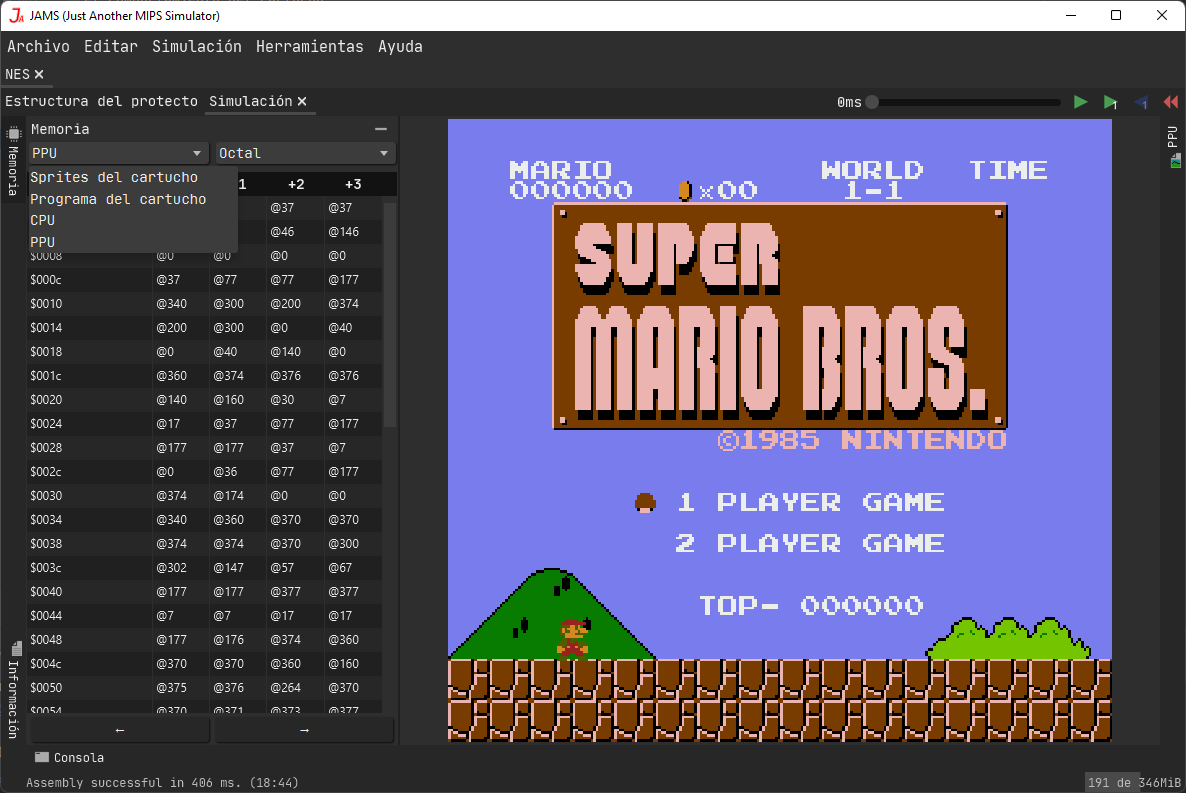
\includegraphics[width=0.8\textwidth]{images/nes/nes-memory}
    \caption{Memoria del simulador}
    \label{fig:nes-memory}
\end{figure}

La herramienta \textbf{memoria} mostrada en la
figura \ref{fig:nes-memory} permite
al usuario visualizar la memoria del simulador desde
el punto de vista de la \textit{CPU} de la \textit{PPU}.
Adicionalmente, también le permite visualizar los bancos
de memoria del cartucho de forma directa, sin controladores
de memoria de por medio.

El usuario también puede \textbf{escribir} valores en una
dirección de memoria.
Esta escritura se tratará como una escritura de la \textit{CPU}
o la \textit{PPU}, dependiendo del punto de vista seleccionado.
Por este motivo, existen escrituras realizadas desde uno de estos
dos puntos de vista que resultarán \textbf{sin efecto} alguno,
ya que se intentará modificar valores como los bancos de memoria
del cartucho, considerados como memoria de solo
lectura por ambos componentes.
Si el usuario desea modificar los bancos de memoria, puede
hacerlo desde la visualización directa.

\subsection{Unidad de procesamiento de imágenes}\label{subsec:unidad-de-procesamiento-de-imagenes}

La \textit{PPU}\cite{PPU} es la unidad de procesamiento encargada de generar
la salida de vídeo.
Debido a la escasa memoria presente en la \textit{VRAM}, la \textit{PPU}
está diseñada para ahorrar \textbf{la mayor cantidad de memoria posible}.
Esto lo consigue construyendo la escena mediante un complejo
sistema de paletas y tablas de patrones.

\subsubsection{Fondo de la escena}\label{subsubsec:fondo-de-la-escena}

Para generar el fondo de la escena, la \textit{PPU} utiliza
tres bancos de memoria diferentes: las tablas de patrones\cite{PATTERN_TABLES},
las tablas de nombres\cite{NAME_TABLES} y las paletas\cite{PALETTES}.

Las tablas de nombres tienen un tamaño de 32x32 bytes.
Las 30 primeras filas guardan el índice del patrón
utilizado en la posición asignada a dicha dirección.
Las dos últimas filas almacenan el identificador de las
paletas empleado en cada conjunto de 2x2 índices.
De esta manera se genera un escenario de 32x30 patrones.

La \textit{PPU} contiene en su memoria \textbf{dos tablas de nombre}
(comúnmente denominadas \textit{A} y \textit{B}),
aunque tenga reservado direcciones de memoria para cuatro de ellas.
Estas direcciones \textbf{apuntan} a la tabla
\textit{A} o a la tabla \textit{B} dependiendo
del \textbf{modo espejo}\cite{MIRRORING} especificado por el videojuego.
Cabe destacar que existen videojuegos con memoria \textit{RAM}
extra en sus cartuchos, permitiendo añadir las tablas \textit{C} y \textit{D}.
\note{Óscar: ¿para qué sirve todo esto, que pueda acceder a 4 tablas
  de nombres, dos de ellas reflejo de las dos existentes?}

\begin{figure}[h]
    \centering
    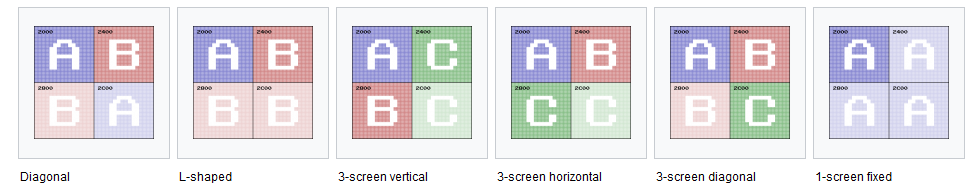
\includegraphics[width=\textwidth]{images/nes/nes-mirroring}
    \caption{Diferentes modos espejo representados en la web \textit{NESdev Wiki}}
    \label{fig:nes-mirroring}
\end{figure}

\begin{figure}[h]
    \centering
    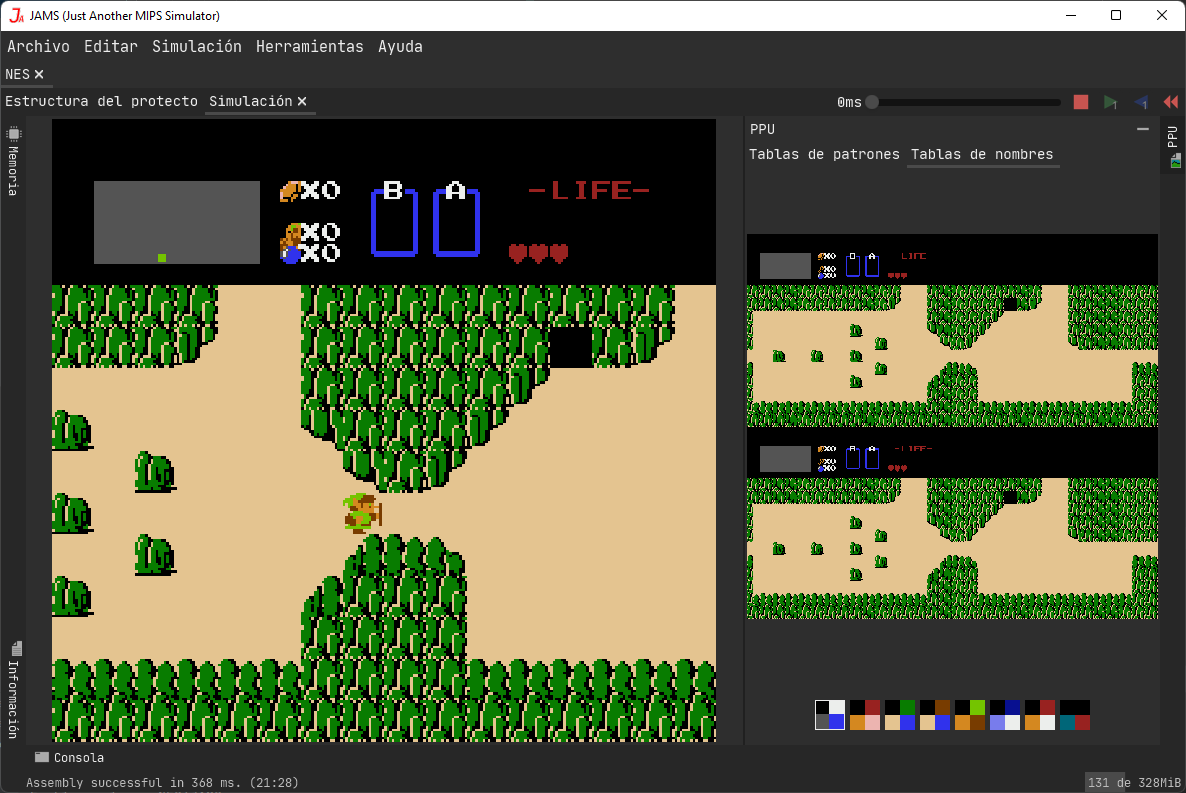
\includegraphics[width=0.8\textwidth]{images/nes/nes-nametables}
    \caption{Tablas de nombres en la herramienta \textit{PPU}}
    \label{fig:nes-nametables}
\end{figure}

Las tablas de patrones permiten guardar 16x16 patrones de
8x8 píxeles cada uno.
Cada pixel ocupa 2 bits de memoria, por lo que una tabla
de patrones ocupa 4 KiB.
La \textit{NES} presenta \textbf{dos tablas de patrones}, siendo
por defecto la primera utilizada para el fondo y la segunda
para los \textit{sprites}.

Por último, la \textit{NES} contiene \textbf{ocho paletas}
de cuatro colores cada una.
Las cuatro primeras paletas se usan para el fondo,
mientras que las cuatro últimas se emplean para los \textit{sprites}.
El primer color de las paletas tiene un comportamiento especial:
en las paletas de fondo, este color siempre es el mismo,
leyendo la \textit{PPU} siempre el color de la primera paleta.
Se considera este color como el color base de la escena.
En las paletas de los \textit{sprites}, el primer color
se considera siempre transparente.

Con esta configuración, la \textit{NES} genera una escena de juego
con un fondo de 512x480 píxeles, cuatro veces mayor que la salida
de vídeo de la consola.
La \textit{PPU} permite a los videojuegos desplazar la salida
de vídeo por la escena con una precisión de píxel.
Si el desplazamiento es tan grande que el área de renderizado
sale de la escena, se produce un desbordamiento en la \textit{PPU},
de forma que la tabla de nombres actúa como una memoria circular
y se dibuja en pantalla el fragmento de la escena que está en el lado contrario.
Gracias a estas propiedades se puede crear videojuegos con
un desplazamiento suave y fácil de implementar.

\subsubsection{\textit{Sprites}}\label{subsubsec:sprites}

La \textit{PPU} contiene una memoria exclusiva para guardar
los atributos de los \textit{sprites}.
Esta memoria recibe el nombre de \textit{OAM} u \textit{Object Attribute Memory}\cite{OAM},
y es capaz de almacenar hasta 64 \textit{sprites}.
Cada \textit{sprite} ocupa 4 bytes de memoria, donde se
definen atributos como el índice del patrón o la posición en la escena.

Cabe destacar la posición de los \textit{sprites} es
absoluta con respeto a la salida de vídeo, por lo que no
es afectada por el desplazamiento del fondo.
Es el propio videojuego el que debe encargarse
de actualizar la posición de todos los \textit{sprites}
cuando la escena se desplaza.

\subsubsection{Herramienta \textit{PPU}}

\begin{figure}[h]
    \centering
    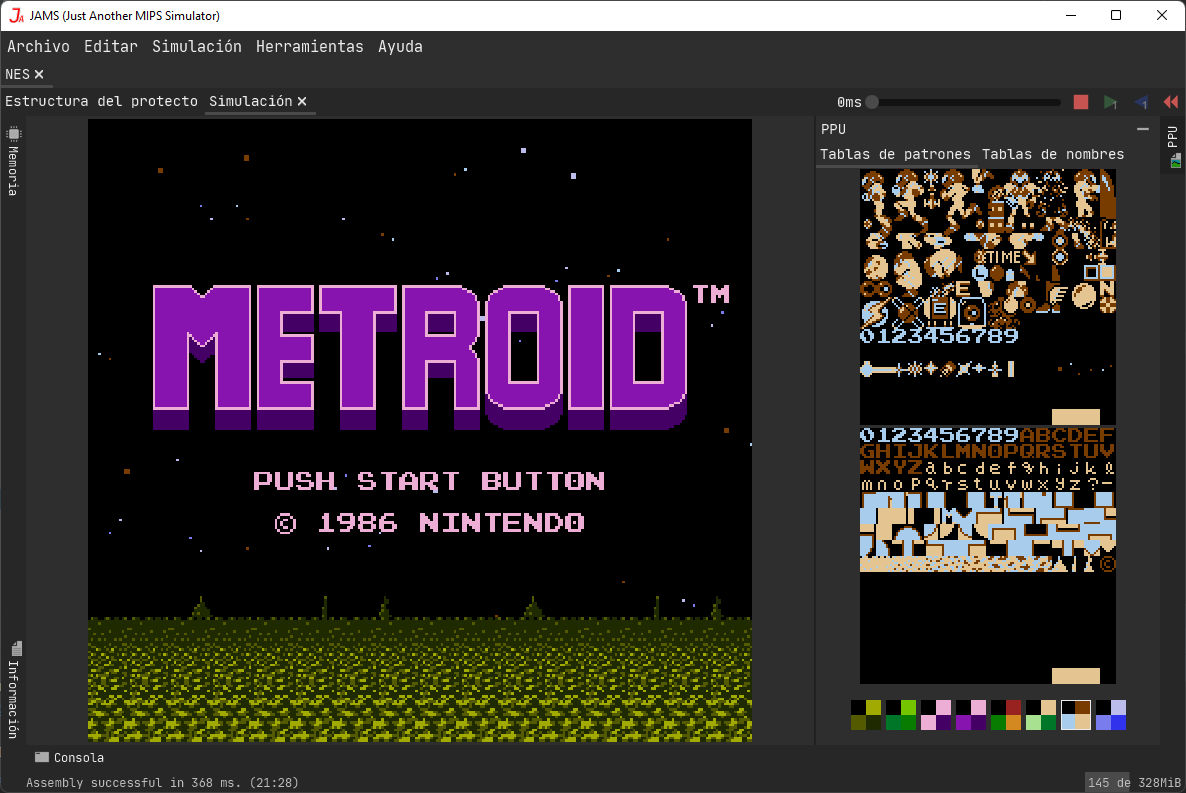
\includegraphics[width=0.8\textwidth]{images/nes/nes-patterntables}
    \caption{Paletas y tablas de patrones en la herramienta \textit{PPU}}
    \label{fig:nes-patterntables}
\end{figure}

La herramienta \textbf{PPU} del simulador permite
visualizar las tablas de patrones, las tablas de nombres
y las paletas que residen actualmente en memoria.
Estos datos se actualizan \textbf{en cada fotograma},
lo que permite detectar los cambios en la \textit{PPU}
de una manera muy visual.
Las figuras \ref{fig:nes-nametables} y \ref{fig:nes-patterntables}
muestran las diferentes opciones de esta herramienta.

Cabe destacar que esta herramienta no es puramente visual:
el usuario puede seleccionar una paleta de la lista.
Esto hará que las tablas de patrones \textbf{usen la paleta seleccionada}.
Muchos videojuegos modifican algunas paletas cada poco tiempo
para crear pequeñas animaciones.
Este es el caso de las monedas en \textit{Super Mario Bros.}, que
cambian de color cíclicamente.
Si la paleta seleccionada está siendo animada, las tablas de patrones
cambiarán de color de forma alternativa.

\subsection{Audio}\label{subsec:audio}

La consola \textit{NES} presenta
una \textbf{unidad de procesamiento de audio} o \textit{APU}\cite{APU}.
Esta unidad tiene \textbf{cuatro canales}: dos canales de pulso,
un canal triangular y un canal de ruido.

En la consola original, los cuatro canales generaban una muestra
por cada ciclo de reloj de la \textit{CPU}, lo que equivaldría
a \textbf{1,77 millones de muestras por minuto}.
Esta cantidad de muestras es innecesaria en un equipo de sonido
moderno, y su reproducción resulta inviable en las librerías
modernas.
Por ello \textit{NES4JAMS} rebaja la cantidad de datos comprimiendo
todas las muestras de un periodo de tiempo en una media ponderada.

\subsection{Unidad de procesamiento central}\label{subsec:unidad-de-procesamiento-central}

Como elemento final del simulador se encuentra el componente
principal de la consola: la \textbf{unidad de procesamiento central}
o \textit{CPU}.
La \textit{NES} usa un procesador \textit{MOS 6502}\cite{MOS6502}: una unidad
de procesamiento central de 8 bits muy utilizada a principio
de los años 80.

Aunque el número de instrucciones documentadas por \textit{MOS Technologies}
sea de 151, existen \textbf{instrucciones no oficiales}, producto del diseño
del procesador, lo que aumenta el número de instrucciones a 256.
\textit{NES4JAMS} actualmente \textbf{no soporta} este tipo de instrucciones,
lo que puede impedir simular ciertos juegos las utilizan.


    \clearpage{\pagestyle{empty}\cleardoublepage}

    \chapter{Resultados}\label{ch:resultados}


\section{Resultados relativos al objetivo 1}\label{sec:resultados-relativos-al-objetivo-1}

Los resultados de este objetivo corresponden al desarrollo
de un \textbf{sistema de vinculación de componentes} para el
entorno de desarrollo integrado \textit{JAMS},
permitiendo a otros desarrolladores aportar nuevas funcionalidades
a la aplicación de manera sencilla.

Este objetivo se ha conseguido, ya que el sistema de
vinculación de componentes desarrollado permite
instalar y desinstalar componentes sin que el usuario tenga
que reiniciar la aplicación.
Además, mediante el sistema de dependencias débiles y fuertes,
los componentes pueden \textbf{interactuar entre sí}, añadiendo
más flexibilidad a los desarrolladores.

\begin{figure}[h]
    \centering
    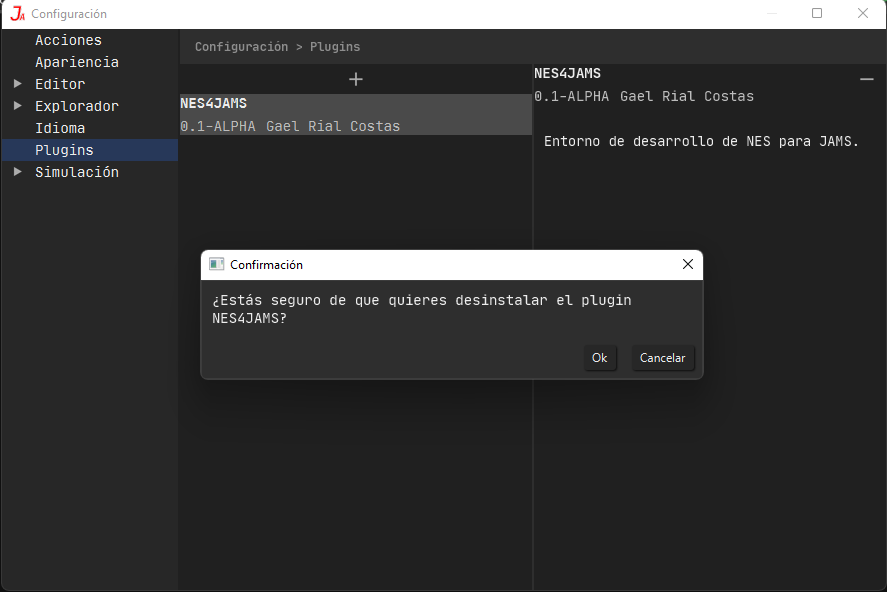
\includegraphics[width=0.8\textwidth]{images/results/jams-uninstall}
    \caption{Desinstalación de un componente}
    \label{fig:jams-uninstall}
\end{figure}

El hecho de que \textit{JAMS} esté escrito en \textit{Java}
ha permitido simplificar mucho el desarrollo de este sistema
de vinculación.
Gracias a las librerías presentes en el \textit{JDK} para cargar
código externo, \textit{JAMS} puede gozar de un sistema de componentes
muy sólido.

El sistema de \textbf{proveedores} desarrollado para los elementos
proporcionados por los componentes también ha resultado ser un éxito.
Este sistema permite que ninguna referencia a ninguna clase de un
componente quede referenciada en \textit{JAMS} cuando dicho componente
se desinstala.
Sin el sistema de proveedores, la desinstalación sería imposible debido
a los errores que se podrían producir.


\section{Resultados relativos al objetivo 2}\label{sec:resultados-relativos-al-objetivo-2}

Los resultados de este objetivo corresponden al desarrollo y mejora de
\textbf{diversas tecnologías} para permitir a los componentes modificar
todos los aspectos de \textit{JAMS} de una manera rápida y sencilla.

Este objetivo también se ha alcanzado.
La tecnología desarrollada más usada por los componentes
y por el propio \textit{JAMS} es el sistema de \textbf{gestores},
que ha permitido gestionar los elementos de la aplicación
de una manera rápida y sencilla, haciendo que los componentes
puedan añadir nuevos elementos de forma transparente.
Este sistema se complementa con los \textbf{eventos},
que permiten recibir información sobre los sucesos
acontecidos en el entorno de desarrollo.
Combinando ambos sistemas, tanto \textit{JAMS} como los componentes
pueden refrescar su información fácilmente cuando se añade o elimina
algún elemento de un gestor.

\begin{figure}[h]
    \centering
    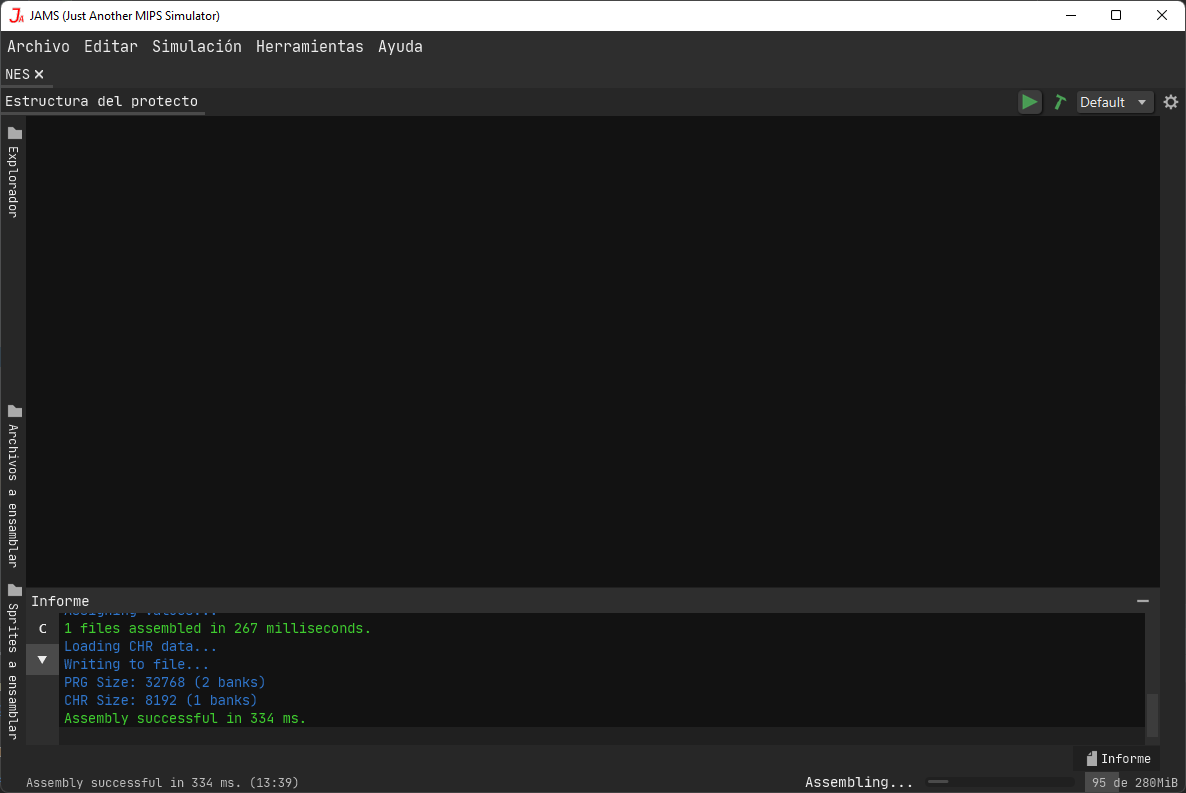
\includegraphics[width=0.8\textwidth]{images/results/jams-tasks}
    \caption{Barra de tareas informando sobre el ensamblaje}
    \label{fig:jams-tasks}
\end{figure}

Otra tecnología muy utilizada han sido las \textbf{tareas},
que permiten ejecutar código asíncrono de una manera muy
sencilla.
Gracias a tener todas las tareas de un proyecto agrupadas
en un ejecutor, se ha podido añadir
un elemento en la barra inferior de la aplicación que muestra
el proceso de todas las tareas del proyecto actual,
tal como se muestra en la figura \ref{fig:jams-tasks}.


\section{Resultados relativos al objetivo 3}\label{sec:resultados-relativos-al-objetivo-3}

Los resultados de este objetivo corresponden al desarrollo
de un componente que añada a \textit{JAMS} un \textbf{entorno de
desarrollo integrado} para la creación de videojuegos de la
consola \textit{NES}, incorporando un editor de código
y de gráficos, un ensamblador y un simulador.

Este objetivo también se considera superado de manera satisfactoria.
El nuevo componente permite desarrollar videojuegos de
la \textit{NES} usando un editor de código muy similar al del
entorno de desarrollo para \textit{MIPS32}, incorporando
herramientas como el \textbf{autocompletador} o el \textbf{inspector de código},
que permite agilizar el desarrollo de los videojuegos.
El componente también presenta un editor de gráficos, que permite
editar los patrones presentes en las tablas del juego.

\begin{figure}[h]
    \centering
    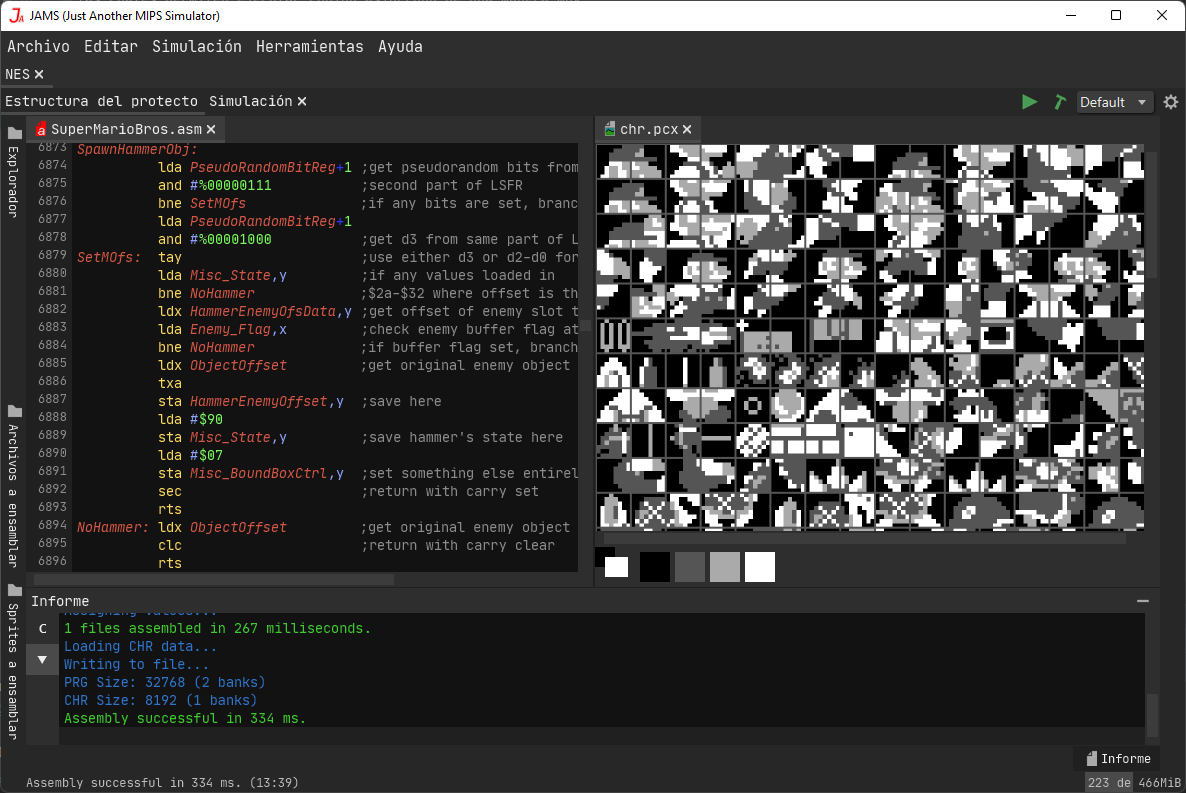
\includegraphics[width=0.8\textwidth]{images/results/nes-editor}
    \caption{Editor de código y de gráficos}
    \label{fig:nes-result-editor}
\end{figure}

El ensamblador, inspirado por el ensamblador presente
en \textit{JAMS} para la arquitectura \textit{MIPS32},
incorpora varias características avanzadas no encontradas
en ensambladores más sencillos, como lo son las referencias
relativas o las macros anidadas.
Este ensamblador escribe el resultado en un archivo \textit{iNES},
lo que permite al desarrollador distribuir su videojuego de manera
sencilla.

Por último, \textit{NES4JAMS} incorpora un simulador de la arquitectura
de la consola \textit{NES} que permite ejecutar la mayoría de los
videojuegos comerciales.
Este simulador permite visualizar el estado del videojuego desde varios
puntos de vista gracias a las herramientas incluidas.
La herramienta más característica del simulador es la herramienta
\textit{PPU}, que presenta de manera muy visual el estado
de la unidad de procesamiento de imágenes,
como se observa en la figura \ref{fig:nes-result-simulator}.

\begin{figure}[h]
    \centering
    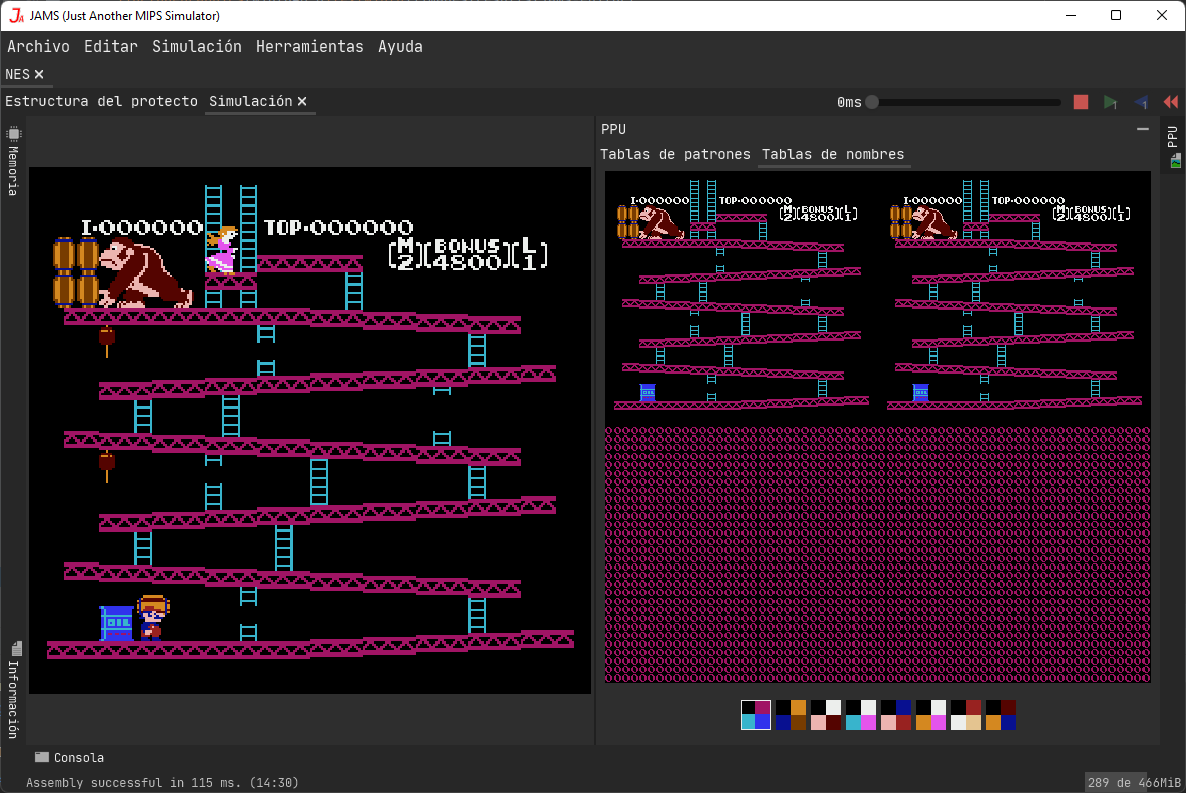
\includegraphics[width=0.8\textwidth]{images/results/nes-simulator}
    \caption{Simulador con la herramienta \textit{PPU}}
    \label{fig:nes-result-simulator}
\end{figure}

Todos estos elementos conforman un entorno de desarrollo
\textbf{sólido} para la creación de nuevos videojuegos
para la \textit{NES}.

Por último, cabe destacar que la elección del lenguaje
de programación \textit{Kotlin} para el desarrollo de
este componente ha sido una totalmente adecuada.
Su diseño más conciso, combinado con nuevas características
como el soporte para números sin signo, ha permitido
acelerar el ritmo de desarrollo del componente.
La capacidad de \textit{Kotlin} de permitir ejecutar sus
programas en la \textit{JVM} permite que se puedan
crear componentes para \textit{JAMS} en este lenguaje
de programación de manera \textbf{transparente}, sin
que el desarrollador tenga que ejecutar ningún paso intermedio.

    \clearpage{\pagestyle{empty}\cleardoublepage}

    \chapter{Conclusiones}\label{ch:conclusiones}

Los objetivos de este proyecto estaban asociados
a la \textbf{creación de un sistema de componentes}
para el entorno de desarrollo \textit{JAMS}, permitiendo
a otros desarrolladores expandir las características
de la aplicación.

\textit{JAMS} es un entorno de desarrollo moderno,
flexible, modular y fácil de usar, donde el usuario
puede crear aplicaciones de una manera rápida y cómoda.
Las nuevas tecnologías desarrolladas en este
Trabajo de Fin de Grado permiten \textbf{mantener esta arquitectura}
flexible y modular, permitiendo a otros desarrolladores
añadir funcionalidades sin tener que modificar el propio
código de la aplicación.

Para probar el funcionamiento de todas estas tecnologías
se ha desarrollado un componente que añade un \textbf{entorno
de desarrollo integrado} para el desarrollo de videojuegos
para la consola \textit{NES}.
Gracias a la creación de este componente, las tecnologías
utilizadas en \textit{JAMS} gozan de una arquitectura
flexible, pero robusta.

\section{Limitaciones}\label{sec:limitaciones}

Las tecnologías desarrolladas en este Trabajo
de Fin de Grado presentan las siguientes limitaciones:

\begin{itemize}
    \item \textbf{Velocidad}: el sistema de eventos
    presenta un rendimiento bastante bajo: el uso
    de este en el simulador \textbf{ralentiza la ejecución
    de manera considerable}.
    La búsqueda de gestores también tiende a ralentizar
    la ejecución de la aplicación.
    \item \textbf{Distribución}: \textit{JAMS} no presenta
    ninguna tenga \note{Óscar: tienes que repasar esta frase} de componentes que permita a los desarrolladores
    publicar sus componentes.
    Los desarrolladores deben publicar sus componentes de manera
    externa a la propia aplicación, lo que puede dificultar
    la distribución de estos.
    \item \textbf{Falta de características}: el simulador
    incluido en el componente \textit{NES4JAMS} sufre
    de una falta de herramientas: los usuarios no son
    capaces de añadir puntos de ruptura o visualizar
    las instrucciones ensambladas de su videojuego.
\end{itemize}

\begin{figure}[h]
    \centering
    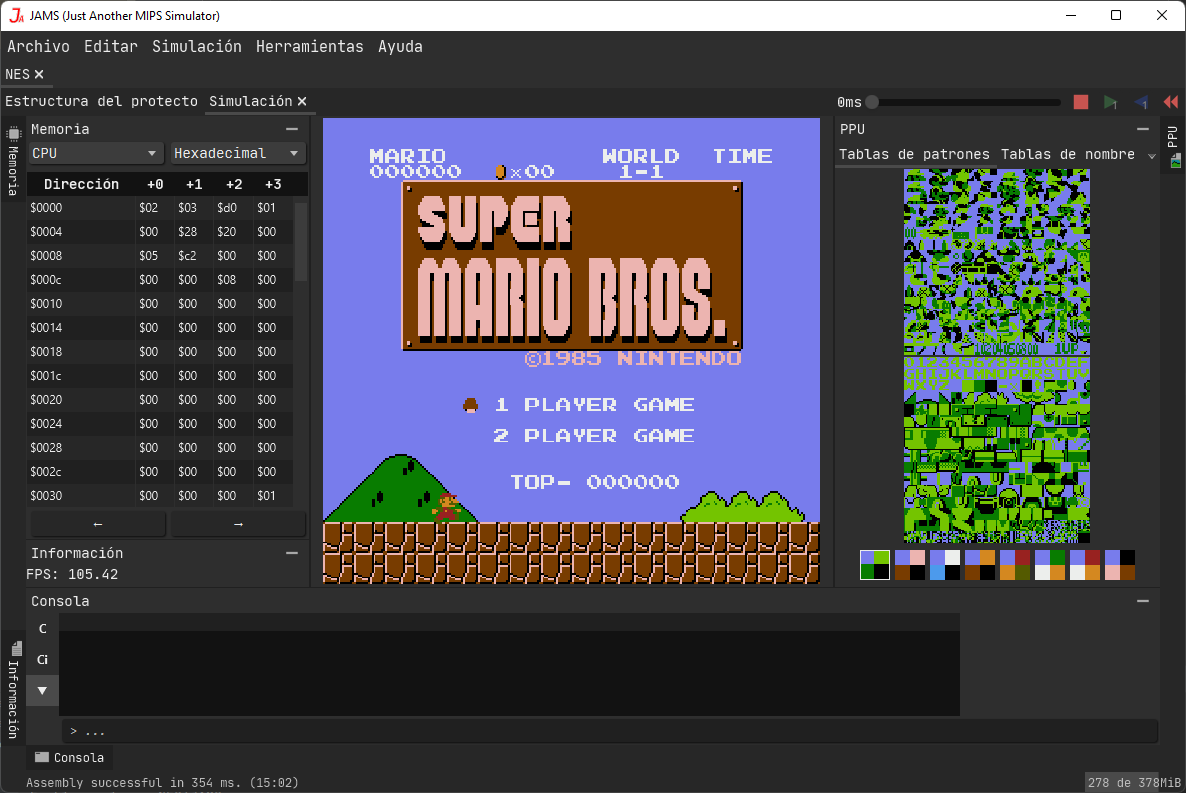
\includegraphics[width=0.8\textwidth]{images/conclusions/nes-simulator-tools}
    \caption{Todas las herramientas presentes en el simulador}
    \label{fig:nes-conclusions-tools}
\end{figure}

\section{Líneas futuras}\label{sec:líneas-futuras}

Tanto \textit{JAMS} como el componente \textit{NES4JAMS}
contarán con varias actualizaciones importantes en
el futuro cercano.

\begin{itemize}
    \item \textbf{Nuevas herramientas para el simulador}:
    como ya se ha mencionado, el simulador presente en
    \textit{NES4JAMS} sufre de una falta de herramientas.
    La primera actualización para el componente añadirá
    nuevas herramientas, como pueden ser un visualizador
    de instrucciones y puntos de ruptura.
    \item \textbf{Uso del \textit{Proyecto Valhalla}:} el
    \textit{Proyecto Valhalla}\cite{PROJECT_VALHALLA}, creado en 2014,
    está desarrollando una de las características más esperadas
    por los desarrolladores \textit{JAVA}: \textbf{paso por valor}.
    Esta característica permitirá optimizar de manera considerable
    todas las herramientas desarrolladas en este Trabajo de Fin
    de Grado.
    Estas nuevas características empezarán su desarrollo cuando esta
    tecnología esté en fase \textit{preview}.
\end{itemize}

\section{Reflexiones finales}\label{sec:reflexiones-finales}

El desarrollo de \textit{NES4JAMS}, junto con el desarrollo
de \textit{JAMS}, ha sido el proyecto más complejo en el
que he trabajado:
este proyecto ha abarcado un montón de conceptos y tecnologías
que hay que sincronizar de manera perfecta para que el resultado
sea robusto.
El desarrollo del sistema de componentes ha resultado en una
vuelta al pasado, donde trabajaba en diferentes expansiones
de videojuegos.

\textit{NES4JAMS} me ha permitido investigar el funcionamiento
de una de las consolas más importantes en la
historia del videojuego.
La capacidad de poder ejecutar videojuegos en una aplicación
desarrollada desde cero ha sido una experiencia muy gratificante.

Finalmente, agradecer a todas las personas que me han
estado apoyando en este proyecto, a mi familia, amigos y a mis
tutores Óscar y Luis, ya que gracias a ellos este trabajo
ha sido posible.

    \clearpage{\pagestyle{empty}\cleardoublepage}

    \backmatter
    \bibliography{main}
    \bibliographystyle{orobles}
    \addcontentsline{toc}{chapter}{Bibliografía}
\end{document}
